\documentclass[a4paper,oneside,12pt]{book} 
 
\usepackage[xetex]{graphicx}
\usepackage{fontspec}
\usepackage{xunicode}
\usepackage{amsfonts}
\usepackage{amsmath}
\usepackage{nicefrac}
%\defaultfontfeatures{Mapping=tex-text,Ligatures={Common}}
\defaultfontfeatures{Mapping=tex-text,Scale=MatchLowercase,Ligatures={Common}}
%\setmonofont{LMMonoLt10}
\setmainfont{Junicode}
%\setromanfont{Latin Modern Roman}
%\setromancapsfont{Latin Modern Roman}
% \setmainfont[
%  BoldFont={Junicode}, 
%  ItalicFont={Junicode},
%  BoldItalicFont={Junicode}
%  ]{Gentium}

%\setromanfont{Times New Roman}
%\setromanfont{DejaVu Serif}
%\setromanfont{Linux Libertine O}
% \setsansfont[Mapping=tex-text]{DejaVu Sans}
% \setmonofont[Mapping=tex-text]{DejaVu Sans Mono}

\newICUfeature{LigType}{disc}{+dlig}

\usepackage{polyglossia}
%\setdefaultlanguage{czech}
\setdefaultlanguage{slovak}
%\PolyglossiaSetup{slovak}{indentfirst=true}

%\usepackage[slovak, english]{babel}
%\usepackage[english,slovak]{babel}

%\usepackage{csquotes}
%\DeclareQuoteStyle{slovak}
%{\quotedblbase}
%{\textquotedblleft}
%[0.05em]
%{\quotesinglbase}
%{\fixligatures\textquoteleft}


\usepackage{url}
\usepackage[xetex]{hyperref}

\usepackage[
   backend=biber      % if we want unicode 
%  ,style=iso-authoryear % iso-authoryear or iso-numeric for numeric citation method
  ,style=authoryear 
%  ,style=authoryear-comp 
  %,babel=other        % to support multiple languages in bibliography
  %,autolang=other % to support multiple languages in bibliography
  ,autolang=langname % to support multiple languages in bibliography
  %,sortlocale=cs_CZ   % locale of main language, it is for sorting
  ,bibencoding=UTF8   % this is necessary only if bibliography file is in different encoding than main document
]{biblatex}
\addbibresource{literatura.bib}

\usepackage{pdfpages}
\usepackage{xcolor}
\usepackage[head=20pt,a4paper]{geometry}
\geometry{top=2.5cm,bottom=2.5cm,left=3.5cm,right=2.0cm}
\usepackage{setspace}
\onehalfspacing
\usepackage{changepage}
\usepackage{indentfirst}

\usepackage{fancyhdr}
\fancypagestyle{plain}{ %
\fancyhf{} %
% \fancyfoot[LE,RO]{\thepage} %
\fancyfoot[RO]{\thepage} %
\renewcommand{\headrulewidth}{0pt} % remove lines as well
\renewcommand{\footrulewidth}{0pt} %
}

%\usepackage{enumerate}
\usepackage{subfig}
\usepackage{array}

\usepackage{comment}

\usepackage{pdflscape}

%%definície konštánt a makier
\def \nazovUniverzity{Univerzita Komensk{é}ho v Bratislave}
\def \NazovUniverzity{\textbf{\Large \sc \nazovUniverzity}} %\sc pre smallcaps
\def \nazovFakulty{Fakulta matematiky, fyziky a informatiky}
\def \NazovFakulty{\textbf{\large \sc \nazovFakulty}}
\def \nazovDiela{Efektívne hľadanie minimálne dominujúcej množiny na reálnych sieťach}
\def \NazovDiela{\LARGE{\em \nazovDiela}}
\def \podnazovDiela{nie je}
\def \PodazovDiela{\large{\em \podnazovDiela}}
\def \typPrace{Diplomová práca}
\def \TypPrace{\large{\typPrace}}
\def \autor{Viktor Tomkovič}
\def \veduci{Mgr. Martin Čajági}
\def \rok{2015}
\def \miestoRok{Bratislava, \rok}
\def \cisloOdboru{2511}
\def \katedra{Katedra aplikovanej informatiky FMFI}
\def \odbor{Aplikovaná informatika}
\def \program{Aplikovaná informatika}
\def\citet#1{\textcite{#1}}
\def\citep#1{\parencite{#1}}
%citat: argumenty sú citát a meno autora
\newcommand{\citat}[2]{\begin{flushright}\small\textsl{#1}\\#2\end{flushright}}
%strednp je vystredenie textu na nepárnej strane bez ohľadu na okraje(!!!), parametrom je text
\newcommand{\stredp}[1]{\begin{adjustwidth}{+0.50cm}{+0.00cm} \begin{center} #1 \end{center} \end{adjustwidth}}
%stredp je obdoba predošlého príkazu len pre párne strany
\newcommand{\strednp}[1]{\begin{adjustwidth}{+0.0cm}{+0.50cm} \begin{center} #1 \end{center} \end{adjustwidth}}
\def\todo#1{\par\smallskip{\scriptsize {\bf TODO: }#1}\par\smallskip}

\setlength\fboxsep{0pt}
\setlength\fboxrule{0.5pt}
\definecolor{grey}{gray}{0.6}
\newcommand{\mybox}[2]{{\color{#1}\fbox{\normalcolor#2}}}
\newcommand{\greybox}[1]{\mybox{grey}{#1}}

% \setlength{\parindent}{0.5in}
% \setlength{\parskip}{0.45cm}
\setlength{\parindent}{0.25in}
%\setlength{\parskip}{0.3em}

\newcommand{\mnn}{\mathbb{N}}
\newcommand{\mnz}{\mathbb{Z}}
\newcommand{\mnr}{\mathbb{R}}
\newcommand{\eul}{e}

\DeclareMathOperator*{\argmax}{arg\,max}
\DeclareMathOperator*{\argmin}{arg\,min}

\def\Java{\texttt{JAVA}}
\def\cpp{\texttt{C++}}


\def\uv#1{„#1“}
\catcode`\"=\active \def "{\begingroup„\def "{\endgroup“}}
\begin{document}
\frontmatter
\pagestyle{plain}
\thispagestyle{empty}
\noindent
\strednp{
\NazovUniverzity\\
\NazovFakulty}
\vfill
\strednp{
\NazovDiela
%% \centerline{\PodazovDiela}
\mbox{}\\
\bigskip
\TypPrace
}
\vfill
\strednp{\textbf{\rok} \hfill{\textbf{\autor}}}
\newpage

\thispagestyle{empty}
\noindent
\strednp{\NazovUniverzity\\ \NazovFakulty}
\vfill
\strednp{\NazovDiela
%% \centerline{\PodazovDiela}
\mbox{}\\
\bigskip
\TypPrace
}
\vfill
\begin{tabular}{ l l }
\textbf{Študijný program:} & \program\\
\textbf{Študijný odbor:} & \cisloOdboru\ \odbor\\
\textbf{Školiace pracovisko:} & \katedra\\
\textbf{Vedúci práce:} &  \veduci
\end{tabular}
\bigskip\\
\bigskip\\
\bigskip\\
\bigskip\\
\strednp{\miestoRok \hfill{\autor}}
\newpage

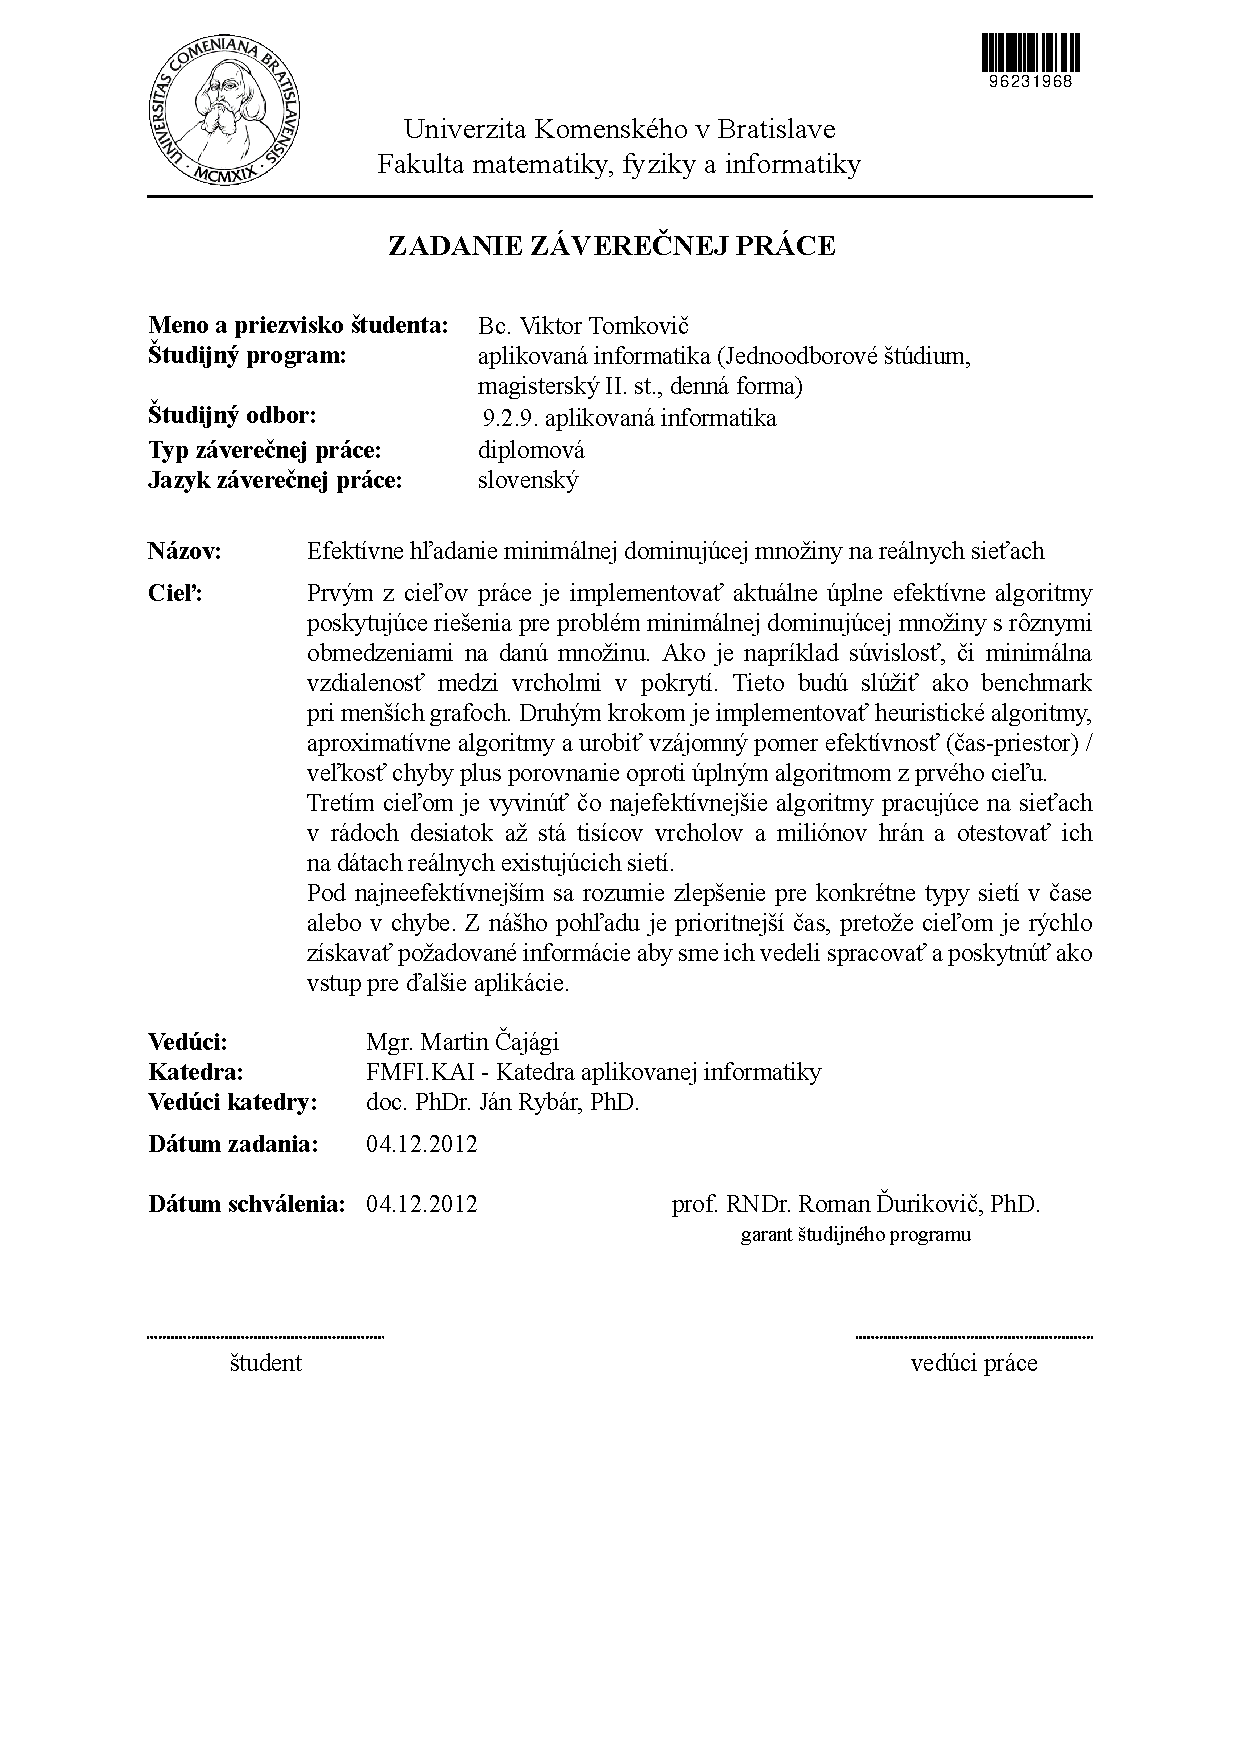
\includepdf[pages=1]{zadanie.pdf}

\newpage

\noindent
~\vfill

\section*{Poďakovanie}
Za odbornú pomoc, poskytnuté materiály a vedenie pri tejto práci patrí vďaka 
môjmu školiteľovi Martinovi Čajágimu. Taktiež by som sa chcel poďakovať 
Marekovi Zemanovi za vedenie jeho kurzom, mojim rodičom za pochopenie a 
poskytnuté možnosti vzdelávať sa a mojim priateľom za podporu.
\\
\bigskip\\
\newpage

\chapter*{Abstrakt}
Veľa reálnych sietí okolo nás má nejakú štruktúru a vlastnosti. Tieto 
vlastnosti sa snažia vedci namodelovať. Úspešne sa to darí sieťami malého 
sveta, bezškálovými sieťami a podobnými modelmi. Často sa pri práci s reálnymi 
sieťami vyskytuje problém nájdenia minimálnej dominujúcej množiny. V tejto 
práci uvádzame prehľad algoritmov na riešenie problému nájdenia minimálnej 
dominujúcej množiny. Ďalej rozoberáme algoritmy, ktoré vedú k lepšiemu 
výsledku, či už časovému alebo priestorovému, na sieťach malého sveta a 
reálnych dátach. Keďže problém je NP-úplný a reálne dáta majú príliš veľa 
vrcholov, venujeme sa najmä heuristikám pažravého algoritmu.\\
Kľúčové slová: minimálna dominujúca množina, MDS, algoritmy a dátové štruktúry, 
siete malého sveta, komplexné siete, pažravý algoritmus.

\newpage

\chapter*{Abstract}
Many real-world networks around us have some structure or features. Scientists 
try to model these features. It is successfully done with small-world networks, 
scale-free networks and with other similar networks. While working with 
small-world networks there often appears the minimum dominating set problem. 
In this work we show the state of current algorithms solving the minimum 
dominating set problem. Further on, we describe algorithms which find better 
results (considering time or set size) on small-world networks and real data. 
Because the problem is NP-complete and the size of real data is big we analyze 
heuristics of basic greedy algorithm.\\
Keywords: minimum dominating set, MDS, algorithms and date structures, small-world 
network, complex networks, greedy algorithm.
\newpage

\mbox{}
\newpage

\tableofcontents
\newpage
%\listoffigures
%\newpage
\listoftables
\newpage

\mainmatter
% \pagestyle{headings}
\pagestyle{fancy}
\fancyhf{} 
% \fancyfoot[LE,RO]{\thepage} 
%  \renewcommand{\chaptermark}[1]{%
% \markboth{\MakeUppercase{%
% \chaptername}\ \thechapter.%
% \ #1}{}}
\renewcommand{\chaptermark}[1]{%
\markboth{\MakeUppercase{%
\chaptername\ \thechapter.%
\ #1}}{}}
% \fancyhead[LE,RO]{\leftmark}
\fancyhead[RO]{\leftmark}
\fancyfoot[RO]{\thepage} 
\renewcommand{\headrulewidth}{0pt} % remove lines as well
\renewcommand{\footrulewidth}{0pt} %
% \renewcommand{\chaptermark}[1]{\markboth{#1}{}} 
% \renewcommand{\sectionmark}[1]{\markright{#1}{}}
\cleardoublepage
% \phantomsection
\addcontentsline{toc}{chapter}{Úvod}
\chapter*{Úvod}\label{chap:intro}

Toto je úvod do mojej diplomovej práce. Bude doplnený neskôr.

\begin{comment}
Ukážka nášho softvéru \emph{Gnarley Trees} je na obrázku~\ref{img:historia}.
Tento projekt začal ako bakalárska práca Jakuba Kováča \citep{kuko};
v tejto práci popisujeme nové dátové štruktúry, ktoré sme vizualizovali
a nové funkcie a vylepšenia, ktoré sme doplnili. Konkrétne ide o 
\emph{union-find problém}, \emph{písmenkový strom (trie)} a 
\emph{sufixový strom}. 

Softvér v súčasnosti vyvíja okrem Kuba Kováča aj Katka Kotrlová, ktorá 
vizualizovala rôzne typy háld a intervalové stromy, Táňa Tóthová, ktorá 
vizualizovala \emph{finger tree} a \emph{B$^+$-strom}.
Okrem vizualizácie softvér prerábame a neustále vylepšujeme.
Pavol Lukča ho doplnil o históriu krokov a operácií. Softvér je celý v 
slovenčine aj angličtine a je 
implementovaný v jazyku \Java. Dostupný je na stránke
{\url{http://people.ksp.sk/~kuko/gnarley-trees}} vo forme appletov
s jednotlivými dátovými štruktúrami, a tiež vo forme samostatného programu,
ktorý obsahuje všetky dátové štruktúry a je určený na používanie offline.

Našou snahou je vytvoriť kvalitný softvér nezávislý od operačného systému, 
ktorý bude vyhovovať ako pomôcka pri výučbe ako aj pri samoštúdiu a bude
voľne prístupný. 

%\bigskip
Predchádzajúci výskum v oblasti pedagogiky
zatiaľ nedokázal úplne preukázať pedagogickú efektívnosť
vizualizácií \citep{shaffer}, avšak viacero štúdií potvrdilo zvýšený záujem
a zapojenosť študentov \citep{naps02, hundhausen02}.

Rozmach vizualizácie algoritmov priniesla najmä \Java\ a jej fungovanie 
bez viazanosti na konkrétny operačný systém. Kvalita iných existujúcich 
vizualizácií sa líši a keďže ide o ľahko naprogramovateľné programy, je ich 
veľa a sú pomerne nekvalitné \citep{shaffer}. 
Zbieraním a analyzovaním kvality sa venuje skupina AlgoViz (\hbox{\url{http://algoviz.org/}}).

Zaujímavé je pozorovanie, že určovanie si vlastného tempa pri vizualizácií 
je veľká pomôcka. Naopak, ukazovanie pseudokódu alebo nemožnosť určenia si
vlastného tempa (napríklad animácia bez možnosti pozastavenia), takmer 
žiadne zlepšenie neprináša \citep{shaffer,saraiya}.

%\bigskip
% Zvyšok článku je organizovaný nasledovne: V sekcií 2 popisujeme implementované
% vylepšenia týkajúce sa vizualizácie, grafiky a ovládania, v sekciách 3 až 6
% nové dátové štruktúry, ktoré sme implementovali a vizualizovali: vyvážené
% stromy, haldy, union-find a písmenkové stromy.

Prácu sme rozdelili na popis jednotlivých dátových štruktúr, ktoré sme 
vizualizovali a popis samotného softvéru. V kapitolách~
\ref{chap:uf}, \ref{chap:trie} a \ref{chap:sx} je postupne popis 
\emph{union-find}, \emph{písmenkového stromu} a \emph{sufixového stromu}. 
V~kapitole~\ref{chap:popis} je popis softvéru a 
v~kapitole~\ref{chap:implementacia} je implementácia.
 
\begin{figure}
\centering
\greybox{%
\includegraphics[width=\columnwidth]{obrazky/gt.png}%
}
\caption{\emph{Softvér Gnarley Trees.} V ovládacom paneli dole môže používateľ
zvoliť operáciu a vstupnú hodnotu a sledovať priebeh algoritmu (zobrazené je vkladanie
prvku 47). Používateľ postupuje vlastným tempom  pomocou tlačidiel \uv{Ďalej} alebo
\uv{Späť}. Vpravo je popis vykonávaných krokov; kliknutím na konkrétny krok v histórií
sa môže používateľ vrátiť.}
\label{img:historia} 
\end{figure}
\end{comment}


\chapter{Definície}\label{chap:definicie}

V tejto kapitole sme zaviedli niektoré pojmy, s ktorými sa budeme stretávať 
počas nasledujúcich kapitol. Sú to prevažne pojmy z teórie grafov. Keďže 
väčšina článkov, ktorými sme sa zaoberali v ďalších častiach je anglického 
pôvodu, rozhodli sme sa pre značenie uprednostniť knihu Graph Theory 
\citep{diestel} pred knihou Grafové algoritmy \citep{plesnik}. 

Základným pojmom je pre nás množina, čo je súbor navzájom rôznych objektov. 
Množinu prirodzených čísel vrátane nuly označujeme $\mnn$. Množinu celých 
čísel označujeme $\mnz$. Množinu reálnych čísel $\mnr$. Pre reálne číslo 
$x$ označujeme hornú celú časť $\lceil x\rceil$ a označuje najmenšie celé 
číslo väčšie alebo rovné ako $x$. Podobne dolnú celú časť označujeme 
$\lfloor x\rfloor$ a označuje najväčšie celé číslo menšie alebo rovné ako $x$. 
Základ logaritmov napísaných ako "$\log$" je 2 a základ logaritmov napísaných 
ako "$\ln$" je $\eul$. Množina $\mathcal = \{A_1, \ldots, A_k\}$ navzájom 
disjunktných podmnožín množina $A$ je \emph{rozdelenie} ak 
$A = \bigcup_{i=1}^{k} A_i$ a všetky $i$ platí, že $A_i = \emptyset$.

\section{Grafy}

Graf $G = (V, E)$ je usporiadaná dvojica množiny vrcholov a množiny hrán, ktorá 
má následujúce vlastnosti: 
\begin{itemize}
	\item $V \cap E = \emptyset$ (hrany a vrcholy sú rozlíšiteľné)
	\item $E \subseteq\left\{ \left\{ u, v\right\} : u \neq v; u, v \in V\right\} $ 
		(hrana spája dva vrcholy)
\end{itemize}

Graf sa zvyčajne znázorňuje nakreslením bodov pre každý vrchol a čiar medzi 
dvoma bodmi tam, kde existuje hrana. Rozmiestenie bodov a čiar nemá význam. 

O grafe s množinou vrcholov $V$ hovoríme, že je grafom \emph{na} $V$. 
\emph{Množina 
vrcholov grafu} $G$ je označovaná $V(G)$ a to aj v prípade, kedy graf $G$ má za 
množinu vrcholov inú množinu ako $V$. Napríklad, pre graf $H = (W, F)$ 
označujeme množinou vrcholov $V(H)$ a platí $V(H) = W$. Podobne označujeme 
\emph{množinu hrán grafu} $E(G)$ (v hore uvedenom príklade platí $E(H) = F$). 
Pre jednoduchosť hovoríme, že vrchol (hrana) patrí grafu a nie množine vrcholov 
(hrán) grafu a preto sa občas vyskytuje označenie $v \in G$ a nie $v \in V(G)$. 

\emph{Rád grafu} je počet vrcholov v grafe a označujeme ho ako $|G|$.
\emph{Prázdny graf} $(\emptyset, \emptyset )$ označujeme $\emptyset$. Grafy 
rádu $0$ alebo $1$ sa označujeme ako \emph{triviálne}.

Vrchol $v$ je incidentný s hranou $e$ ak platí $v \in e$. Hranu $\{x, y\}$ 
jednoduchšie označujeme ako $xy$. \emph{Hranami} $X-Y$ označujeme množinu 
hrán $E(X,Y) = \left\{ \left\{ x, y\right\} : x \in X, y \in Y\right\} $. 
Namiesto $E(\{x\},Y)$ píšeme $E(x,Y)$ a podobne aj namiesto $E(X,\{y\})$ 
píšeme $E(X,y)$. s
Zápisom $E(v)$ označujeme $E(v, V(G))$ a hovoríme o \emph{hranách vrchola} $v$. 

Dva vrcholy $x, y$ grafu $G$ sú \emph{susedia}, ak existuje hrana $xy$ v grafe 
$G$. Dve hrany $e \neq f$ sú susedné, ak majú spoločný jeden vrchol. Ak sú 
všetky vrcholy v grafe navzájom susedné, graf je \emph{kompletný} (alebo 
\emph{úplný}). Kompletný graf s $n$ vrcholmi označujeme $K^n$.

Majme dva grafy $G = (V,E)$ a $G' = (V', E')$. Potom $G \cup G' := (V \cup V', 
E \cup E')$. Podobne $G \cap G' := (V \cap V', E \cap E')$. Ak platí $G \cap G' 
= \emptyset$ tak hovoríme, že grafy sú \emph{disjunktné}. Ak platí $V \subseteq 
V'$ a $E \subseteq E'$, tak potom je graf $G'$ \emph{podgrafom} grafu $G$. 
Zapisujeme $G' \subseteq G$.

Ak $G' \subseteq G$ a $G'$ obsahuje všetky hrany $xy \in E$ pre $x,y \in V'$, 
tak hovoríme, že graf $G'$ je \emph{indukovaný podgraf} grafu $G$. Taktiež 
hovoríme, že $V'$ \emph{indukuje} $G'$ na $G$ a zapisujeme $G' =: G[V']$. 
Zápis $G[\{v\}]$ skracujeme na $G[v]$.

Ak je $U$ nejaká množina vrcholov, tak zápisom $G - U$ (operátory $-$ a 
$\setminus$ budeme občas zamieňať) označujeme $G[V(G) \setminus U]$. Inými 
slovami graf $G - U$ dosiahneme tak, že z grafu $G$ vymažeme všetky vrcholy z 
množiny $U$ a všetky incidentné hrany k nim. Pre $G - \{u\}$ používame aj zápis 
$G - u$.
Pre graf $G=(V,E)$ a množinu hrán $F = \{xy: x, y \in V\}$ zapisujeme 
$G + F = (V, E \cup F)$ a $G - F = (V, E \setminus F)$.

\emph{Komponent grafu} je taký maximálny podgraf, kde medzi každou dvojicou 
vrcholov existuje cesta.

\section{Vlastnosti grafu}

Uvažujme o grafe $G = (V, E)$. Množinu susedov vrchola $v$ označujeme
$N_G(v)$. Pokiaľ to bude z kontextu jasné, tak iba skrátene $N(v)$. Zápis 
rozšírme na množiny. Pre množinu $U \subseteq V$ zapisujeme $N(U)$ množinu 
susedov všetkých vrcholov $u \in U$. Množinu $N(U)$ nazývame \emph{susedmi} $U$. 
\emph{Susedov vrátane vrchola} označujeme susedov vrchola s vrcholom samotným. 
Pre vrchol $v$ susedov vrátane vrchola zapisujeme ako $N[v] := N(v) \cup \{v\}$. 
Podobne môžeme rozšíriť zápis aj na množiny. \emph{Pokrytím} množiny $U 
\subseteq V$ nazývame množinu $N[U] := N(U) \cup U$.

Číslo $d_G(v) = d(v) := |E_G(v)|$ sa nazýva \emph{stupeň} vrchola. Je to počet 
susedov vrchola (neplatí pre digrafy, multigrafy a iné zložité grafy, ktorými 
sa tu však nezaoberáme). Vrchol stupňa $0$ je \emph{izolovaný}. Číslo $\delta 
(G) := min \{d(v), v \in G\}$ je \emph{minimálny stupeň} grafu $G$. Podobne 
číslo $\Delta (G) := max \{d(v), v \in G\}$ je \emph{maximálny stupeň} grafu 
$G$.

\section{Cesta a cyklus}

\emph{Cesta} je graf $P = (V, E)$ v tvare: 
$$ V = \{x_0, x_1, x_2, x_3, \ldots, x_k\} \qquad 
   E = \{x_0x_1, x_1x_2, x_2x_3, \ldots, x_{k-1}x_k\},$$
kde všetky vrcholy $x_i$ sú navzájom rôzne. Vrcholy $x_0$ a $x_k$ sa nazývajú 
\emph{konce} cesty a zvyšné vrcholy sú \emph{vnútorné} vrcholy. Cestu 
zjednodušene označujeme sledom vrcholov: $P = x_0x_1x_2\cdots x_k$. Aj keď 
nevieme rozlíšiť medzi cestami $P_1 = x_0x_1x_2\cdots x_k$ a 
$P_2 = x_kx_{k-1}x_{k-2}\cdots x_0$, často si zvolíme jednu možnosť a hovoríme 
o \emph{ceste z $x_0$ do $x_k$} (v tomto prípade sme si vybrali cestu $P_1$). 
\emph{Dĺžka cesty} je číslo $k$ (cesta môže mať dĺžku 0).

\emph{Cyklus} je cesta $P = (V, E)$ v tvare 
$$ V = \{ x_0, x_1, x_2, x_3, \ldots, x_{k-1}\} \qquad 
E = \{x_0x_1, x_1x_2, x_2x_3, \ldots, x_{k-2}x_{k-1}, x_{k-1}x_0\}$$

O ceste má zmysel hovoriť iba ak $k \geq 3$. \emph{Dĺžka cyklu} je číslo $k$. 
Je to počet vrcholov (a zároveň aj hrán) v grafe.

V nasledujúcej časti si ukážeme dátové štruktúry, s ktorými sme v práci 
pracovali.

\section{Strom}

Graf, ktorý nemá cyklus, sa nazýva \emph{acyklický}. Taktiež sa nazýva aj 
\emph{les}. Les, ktorý má iba jeden komponent sa nazýva \emph{strom}. Takže 
les je graf, ktorého komponenty sú stromy. Často sa nám oplatí poznať 
základné vlastnosti stromu. 
Tie najzákladnejšie sú zároveň aj zameniteľné a ú rôznymi obmenami definície 
stromu.

Následné tvrdenia sú zameniteľné pre graf $T$:
%\begin{enumerate}[(i)]
\begin{enumerate}
	\item \label{itm:strom} graf $T$ je strom;
	\item ľubovoľné dva vrcholy v grafe $T$ sú spojené jedinečnou cestou 
v grafe $T$;
	\item \label{itm:minsuv} graf $T$ je minimálne súvislý -- graf $T$ 
je spojitý, ale graf $T - e$ je nespojitý pre všetky hrany $e \in T$;
	\item graf $T$ je maxmimálne acyklický -- graf $T$ neobsahuje cyklus, 
ale graf $T + xy$ cyklus obsahuje pre ľubovoľné nesusedné vrcholy $x, y \in T$.
\end{enumerate}

Jedinečnú cestu z vrcholu $x$ do vrcholu $y$ v strome $T$ budeme označovať 
$xTy$. Z ekvivalencie bodov \ref{itm:strom} a \ref{itm:minsuv} vyplýva, 
že pre každý spojitý graf platí, že jeho ľubovoľný najmenej spojitý podgraf 
bude strom.

Vrcholy stupňa jeden sa nazývajú \emph{listy}. Každý netriviálny strom má aspoň 
dva listy. Napríklad konce najdlhšej cesty. Jeden zaujímavý fakt -- ak zo 
stromu odstránime list, ostane nám strom.

Občas je vhodne označiť jeden vrchol stromu špeciálne. A to ako \emph{koreň}. 
Koreň potom tvorí základ stromu. Pokiaľ je koreň nemenný, tak hovoríme 
o \emph{zakorenenom strome}. Vybratím koreňa $k$ v strome $T$ nám dovoľuje 
spraviť čiastočné usporiadanie na $V(T)$. Nech $r$ je koreň stromu $T$, 
$r, x, y \in V(T)$, $x \leq y$ a platí, že $x \in rTy$, potom $\leq$ je 
čiastočné usporiadanie na množine $V(T)$. Zakorenené stromy sa zvyknú kresliť 
"po vrstvách", kde je vidieť čiastočné usporiadanie vrcholov.


\section{Bipartitné grafy}

Nech $r \geq 2$ je prirodzené číslo. Graf $G = (V, E)$ sa nazýva 
\emph{r-partitný}, ak môžeme $V$ rozdeliť do $r$ skupín tak, že každá hrana 
má koniec v inej skupine. Z toho vplýva, že vrcholy v jednej skupine nie sú 
susedné. Ak platí, že  $r = 2$, nenazývame graf "2-partitný" ale 
\emph{bipartitný} (i keď obe pomenovania sú správne).

\section{Toky}

Veľa vecí z reálneho sveta sa dá modelovať pomocou grafov alebo štruktúr 
podobných grafom. Ide napríklad o elektrickú rozvodnú sieť, cestnú sieť, 
vlakovú/dráhovú sieť, komunikačnú sieť. Pri týchto znázorneniach vystupujú 
vždy dvojice komunikácií a "križovatiek" (elektrické vedenie s trafostanicami, 
cesty s mestami, dráhy so zástavkami, linky s prepojovacími stanicami). Každá 
komunikácia má svoju kapacitu. V týchto štruktúrach má zmysel sa pýtať otázky, 
ako napríklad koľko veľa prúdu, zásob, dát dokáže prúdiť medzi dvoma vrcholmi. 
V teórii grafov hovoríme o tokoch. 

Konkrétne komunikáciu si môžeme predstaviť ako hranu $e = xy$, ktorá vyjadruje 
aj smer prúdenia. K usporiadanej dvojici $(x, y)$ môžeme priradiť hodnotu $k$ 
vyjadrujúcu kapacitu komunikácie. Znamená to, že $k$ jednotiek môže prúdiť z 
vrcholu $x$ do vrcholu $y$. Alebo usporiadanej dvojici $(x, y)$ môžeme priradiť
zápornú hodnotu $-k$ a to znamená, že $k$ jednotiek prúdi opačným smerom. To 
znamená, že pre zobrazenie $f:V^2\rightarrow\mnz$ (množina V označuje vrcholy), 
bude platiť, že $f(x,y) = -f(y,x)$, keď $x$ a $y$ sú susedné vrcholy.

Keď už máme vrcholy a komunikácie, musíme mať aj \emph{zdroj} vecí, ktoré po 
komunikáciach budú prúdiť a taktiež miesta, z ktorých budú tieto veci odchádzať 
z modelu. Tie sa označujú ako \emph{stoky}. Okrem týchto špeciálnych vrcholov 
platí, že $$\sum_{y\in N(x)}^{}{f(x,y) = 0}$$

Pokiaľ platia pre graf $G := (V, E)$ a zobrazenie $f:V^2\rightarrow\mnz$ 
vlastnosti $f(x,y) = -f(y,x)$ pre susedné vrcholy $x$ a $y$ a pre vrcholy mimo 
zdrojov a stôk, že $\sum_{y\in N(x)}^{}{f(x,y) = 0}$, tak budeme hovoriť o 
\emph{toku} na grafe $G$.

Graf sme si zadefinovali ako štruktúru, ktorá má hrany \emph{neorientované}, 
to znamená, že nevieme rozlíšiť, kde hrana "začína" a kde "končí". Pri tokoch 
sme ale začali rozlišovať túto vlastnosť a tým sa hrany stali 
\emph{orientovanými}. Grafy sa nazývajú neorientované, pokiaľ sú aj ich hrany 
neorientované a naopak, ak sú orientované hrany, tak hovoríme aj o 
orientovanom grafe. V ďalšom texte budeme orientovanosť uvádzať iba vtedy, keď 
nebude jasne vyplávať z kontextu.

\section{Komplexné siete}

Ďalšie veci, ktoré môžeme pri modelovaní sietí z reálneho sveta skúmať sú 
veci ohľadne štruktúry. Má zmysel sa pýtať na to, aký je priemer grafu, či vieme 
určiť hierarchiu vrcholov a jej, aké komunikácie treba prerušiť na to, aby 
sa sieť rozpadla, kam treba nasadiť obmedzený počet špiónov, aby sme získali čo 
najviac informácií a podobne.

Týmito a následujúcimi záležitosťami sa autor v knihe Graph Theory nezaoberá. 
Preto sa od tejto knihy odkloníme a budeme čerpať z dizertačnej práce, ktorú 
napísal Peter \citet{nather}.

Pri modeloch reálnych sietí má zmysel zaoberať sa nielen stupňami jednotlivých 
vrcholov ale aj distribúciou stupňov a priemerným stupňom vrchola. 
\emph{Priemerný stupeň grafu} $G = (V, E)$ označujeme $\overline{d_G} = \bar{d}$ a 
vypočítame ako: $$\overline{d_G} = \bar{d} = \frac{\sum_{v \in V}^{}{d_v}}{|V|}$$

K zadefinovaniu distribúcie budeme potrebovať ešte jednu funkciu. Táto funkcia 
vracia hodnotu 1 v bode 0 a vo všetkých ostatných bodoch vracia hodnotu 0. 
Takže dobre slúži ako filter. Označme ju $\tau$ a zadefinujme: 
$$\tau (n) = \begin{cases}
\hfill 1 \hfill & \text{ak $n=1$} \\
\hfill 0 \hfill & \text{inak} \\
\end{cases}$$

\emph{Distribúcia stupňov vrcholov} grafu $G$ je funkcia 
$p(d)$ reprezentujúca pravdepodobnosť toho, že vrchol má stupeň $d$. Platí, že: 
$$p(d) = \frac{\sum_{v \in V}^{}{\tau(d - d_v)}}{|V|}$$

Suma vo funkcii prechádza všetkými vrcholmi a vďaka filtračnej funkcii $\tau$ 
spočíta, koľko je vrcholov stupňa $d$. Potom sa toto číslo predelí počtom vrcholov.

Zaujímavou vlastnosťou grafu je \emph{klasterizačný koeficient vrchola}. Je 
definovaný ako pomer počtu hrán medzi susediacimi vrcholmi daného vrchola a 
všetkými možnými (aj potenciálnymi) hranami medzi susediacimi vrcholmi. 
Formálne, pre graf $G := (V, E)$ je \emph{klasterizačný koeficient} vrchola 
$v$ hodnota: $$c_v = \frac{|E(N[v])|}{\binom{|N[v]|}{2}}$$

\emph{Priemerný klasterizačný koeficient} $\bar{c}$ grafu $G$ je definovaný ako:
$$\bar{c} = \frac{\sum_{v\in V}^{c_v}}{|V|}$$

Podobne ako distribúciu stupňov vrcholov zadefinujeme aj distribúciu 
klasterizačných koeficientov. \emph{Distribúcia klasterizačných koeficientov 
grafu} $G$ je funkcia $c(d)$, ktorá hovorí o tom, aký je priemer
klasterizačných koeficientov pre všetky vrcholy stupňa $d$. Vypočítame ho ako: 
$$c(d) = \frac{\sum_{v \in V}^{}{\tau(d - d_v)c_v}}
{\sum_{v \in V}^{}{\tau(d - d_v)}}$$

\section{Vlastnosti komplexných sietí}

V predošlej časti sme uviedli definície vlastností, ktorými vieme medzi sebou 
jednotlivé siete porovnávať a odlíšiť ich od seba.

Prvou vlastnosťou, ktorou môžeme grafy porovnávať a objavuje sa v reálnych 
sieťach, je to, čomu sa hovorí \emph{malý svet}. Graf je sieťou malého sveta 
vtedy, keď je jeho priemer malý a zároveň má vysokú klasterizáciu vrcholov.

Veľa z reálnych sietí má ďalšiu spoločnú vlastnosť. Ich distribúcia stupňov 
vrcholov klesá mocninovo. Môžeme zapísať, že pre distribúciu platí:
$$p(d) = d^{-\alpha}$$

Siete sa líšia v konštante $\alpha$, ale iba trochu. V drvivej väčšine platí, 
že $2 \leq \alpha \leq 3$. Keďže v takýchto sieťach by mal náhodný "výsek" 
grafu podobné vlastnosti, tak táto vlastnosť sa nazýva aj \emph{bezškálovosť}.

\section{Modely sietí}

V tejto časti si ukážeme spôsob vytvárania grafov s nejakou vlastnosťou. Keďže 
sa zaoberáme porovnávaním "obyčajných" grafov so sieťami malého sveta, 
zameriame sa najmä na tieto dva typy.

\emph{Náhodné grafy} môžeme vytvoriť napríklad týmito dvoma spôsobmi. Prvým je, 
že pevne určíme, koľko bude mať graf vrcholov a určíme, koľko hrán má mať graf. 
Potom náhodne vyberieme počet určených hrán. Druhým spôsobom je, že pevne 
určíme počet vrcholov grafu a pravdepodobnosť, s ako sa každá hrana vyberie. 
Grafy vytvorené týmito postupmi nepopisujú (nemajú dostatočné vlastnosti) siete 
malého sveta dostatočne, preto ich nebudeme považovať za siete malého sveta.

\emph{Barabási -- Albertov model} alebo aj model s preferenčným napájaním je 
spôsob vytvárania grafov, ktorý zohľadňuje stupeň vrcholov grafu. Na začiatku 
má graf daný počet náhodne spojených vrcholov a v každom kroku sa pridá 
jeden vrchol a niekoľko hrán spájajú tento pridaný vrchol s existujúcimi 
vrcholmi v grafe. Pravdepodobnosť toho, že sa hraná spojí s vrcholom je priamo 
úmerná stupňu vrchola. Tento postup vedie ku tvorbe grafom podobným 
vlastnosťami s komplexnými sieťami.

\section{Asymptotická zložitosť}

V tejto práci sa zaoberáme najmä prácou s reálnymi dátami a konkrétnymi 
algoritmami. Ale aj pri tomto zameraní je dobre, keď vieme približne odhadnúť 
s akými veľkými množstvami dát algoritmus pracuje, ako zhruba veľa operácií 
procesor vyžaduje na daný výpočet v závislosti od veľkosti vstupných dát. Inými 
slovami, potrebujeme buď vedieť porovnať dve funkcie alebo nejakú funkciu 
zatriediť medzi ostatné. 

Na tieto požiadavky vznikla \emph{"O-notácia"} \citep{onot}, ktorá vyjadruje 
asymptotický rast funkcií. Uplatňuje sa v informatike a matematike. 
Ide o vytvorenie rôznych tried funkcií. Aj keď v informatike sa zväčša 
porovnáva rast počtu krokov od veľkosti vstupu a veľkosť vstupu aj počet krokov 
sú diskrétne údaje, uvedieme tu definíciu pre funkcie, ktoré majú svoj 
definičný obor aj obor hodnôt v množinách reálnych čísel.

Vyjadrime \emph{asymptotický odhad zhora}. 
Majme dve funkcie $f, g: \mnr \rightarrow \mnr$. Potom:

$$\exists c\ge 0\ \exists x_0\ \forall x\ge x_0: 
f(x) \leq c\cdot g(x) \iff f(x) \in O(g(x))$$

Veľmi často sa v informatike zamieňa zápis $f(x) \in O(g(x))$ so zápisom 
$f(x) = O(g(x))$ a hovorí sa, že "$f(x)$ je $O(g(x))$". Napríklad, ak 
funkcia $f(x) = 5x^2+3x+7$ a funkcia $g(x) = x^2$, tak sa hovorí, 
že "$f(x)$ je $O(x^2)$". Taktiež môžeme povedať, že $f(x)$ rastie 
kvadraticky.

Vidno, že funkcia $g(x)$ nejakým spôsobom ohraničuje funkciu $f(x)$ zhora. 
Asymptotický odhad pomocou $O(g(x))$ nám ale nehovorí nič o tom, ako veľmi 
zhora je funkcia $f(x)$ ohraničená. Zväčša sa však používa dostatočne tesný 
odhad.

Ak však chceme byť v našom odhade presnejší, existuje aj \emph{asymptoticky tesný 
odhad} a je definovaný ako:

$$\exists c_1\ge 0\ \exists c_2\ge 0\ \exists x_0\ \forall x\ge x_0: 
c_1\cdot g(x)\leq f(x) \wedge f(x) \leq c_2\cdot g(x) \iff f(x) \in \Theta (g(x))$$

V praxi sa používa menej. Je však vhodný, ak chceme ukázať najtesnejší odhad 
pre daný algoritmus. Ak existuje. Ak neexistuje, alebo sme ho zatiaľ nenašli, 
tak neostáva nič iné, ako spraviť tesný horný a dolný odhad. 
\emph{Asymptotický dolný odhad} je 
definovaný ako:

$$\exists c\ge 0\ \exists x_0\ \forall x\ge x_0: 
c\cdot g(x) \leq f(x) \iff f(x) \in \Omega (g(x))$$

Z tejto definície je vidieť, že \emph{asymptoticky tesný odhad} $\Theta (g(x))$ 
môžeme vyjadriť aj ako: 

$$f(x) \in O(g(x)) \wedge f(x) \in \Omega (g(x)) \iff f(x) \in \Theta (g(x))$$

Tento vzťah dobre vyjadruje reálnu snahu pri určovaní asymptotickej zložitosti 
algoritmov. Algoritmus sa hrubo odhadne zhora aj zdola a postupne sa tieto 
odhadu spresňujú. 

V matimatike sa používa ešte jeden asymptotický vzťah a to 
\emph{asymptotická rovnosť}. Je to podobný vzťah ako tesný asymptotický odhad, 
opäť používa dve funkcie $f(x), g(x)$ na reálnych číslach a je definovaný ako:

$$\forall \varepsilon \ge 0 \exists n_0 \forall n > n_0: 
\left| \frac{f(x)}{g(x)} - 1 \right| < \varepsilon \iff f(x) \sim g(x)$$

Z definície je vidieť, že pokiaľ sú dve funkcie asymptoticky rovnaké, tak budú 
aj navzájom asymptoticky tesné.

\section{Ostatné definície}

V tejto časti uvádzame iné definície, o ktorých si myslíme, že sú užitočné.

\emph{Maximum}, respektíve \emph{minimum} funkcie je najväčšia, resp.\ najmenšia 
hodnota, ktorú funkcia nadobúda. Pre funkciu $f(x)$ platí, že: 
\begin{align*}
\max f(x) := f(x) \mid \forall y : f(y) \leq f(x) \\
\min f(x) := f(x) \mid \forall y : f(y) \geq f(x)
\end{align*}

\emph{Argumentom maxima}, respektíve \emph{argumentom minima} funkcie sú prvky 
z definičného oboru funkcie, v ktorom funkcia nadobúda maximum, resp.\ minimum. 
Pre funkciu $f(x)$ platí, že: 
\begin{align*}
\argmax_x f(x) := \left\{x \mid \forall y : f(y) \leq f(x)\right\} \\
\argmin_x f(x) := \left\{x \mid \forall y : f(y) \geq f(x)\right\}
\end{align*}

V následujúcich kapitolách sme sa zamerali a prebrali si jednotlivé existujúce 
algoritmy, ktoré boli implementované.

\chapter{Prehľad algoritmov}\label{chap:algoritmy}

V tejto kapitole si spravíme prehľad algoritmov, ktoré existujú na nájdenie 
minimálnej dominujúcej množiny. Najprv zadefinujeme minimálnu dominujúcu 
množinu, neskôr určíme požiadavky na algoritmy a potom popíšeme jednotlivé 
konkrétne algoritmy.

\section{Dominujúce množiny}

\emph{Dominujúca množina} $S$ na grafe $G = (V, E)$ je podmnožina množiny 
vrcholov $V$ grafu $G$ taká, že každý vrchol grafu sa v množine nachádza 
alebo je susedný s dominujúcou množinou. Pre množinu platí: $N[S] = V$. 
Z definície je zrejmé, že o dominujúcich množinách má zmysel hovoriť iba pri 
grafoch s konečným počtom vrcholov.

\emph{Minimálna dominujúca množina} $S_M$ je dominujúca množina s najmenšou 
kardinalitou.

\emph{Dominančé číslo} $\gamma (G)$ grafu $G$ je kardinalita minimálnej 
dominujúcej množiny. Ak je množina $S_M$ minimálnou dominujúcou množinou, tak 
platí, že $\gamma (G) = |S_M|$.

Na tomto mieste zadefinujeme aj vrcholové pokrytie. Uvádzame ho tu preto, lebo 
problém nájdenia vrcholového pokrytia súvisí s problémom nájdenia minimálnej 
dominujúcej množiny. \emph{Vrcholové pokrytie} $S^\prime$ na grafe $G = (V, E)$ 
je podmnožina množiny vrcholov $V$ grafu $G$ taká, že každá hrana $xy \in E$ 
je incidentná s vrcholom vrcholového pokrytia. Pre množinu platí: 
$\forall xy \in E: x \in S^\prime \vee y \in S^\prime $

Podobne ako pri minimálnej dominujúcej množine, existuje aj minimálne vrcholové 
pokrytie.

Jedným zo spôsobov, ako vyriešiť problém nájdenia minimálnej dominujúcej 
množiny je previesť ho na problém množinového pokrytia. \emph{Množinové 
pokrytie} je súbor množín, ktorých zjednotenie obsahuje všetky prvky univerza. 
Formálne je daná usporiadaná dvojica $(\mathcal{S}, \mathcal{U})$, kde:

\begin{itemize}
	\item množina množín $\mathcal{S}$ obsahuje množiny $S_1, S_2, S_3, ..., 
		S_n$ také, že $\bigcup_{i = 1}^{n} S_i = \mathcal{U}$;
	\item množina $\mathcal{U}$ je množina všetkých prvkov a nazýva sa 
		\emph{univerzum}.
\end{itemize}

Množinové pokrytie je podmnožina $\mathcal{C} \subseteq \mathcal{S}$ množín, 
pre ktorú platí, že $\bigcup_{C \in \mathcal{C}} C = \mathcal{U}$.

\section{Požiadavky na algoritmy}

Táto práca ma za úlohu nájsť vhodný algorimus na hľadanie minimálnej 
dominujúcej množiny. Ale pre reálne dáta. To znamená, že grafy, na ktorých 
budeme minimálnu dominujúcu množinu hľadať majú veľa vrcholov. Avšak problém 
nájdenia minimálnej dominujúcej množiny na grafe sa dá redukovať na problém 
vrcholového pokrytia, o ktorom vieme, že je NP-ťažký. To znamená, že na 
vyrátanie minimálnej dominujúcej množiny treba veľmi veľa výpočtového času na 
súčasných počítačoch. Keďže pre reálne požiadavky je častokrát lepší nejaký, 
aj keď nie optimálny výsledok, tak sme sa rozhodli, že algoritmus nemusí dávať 
optimálny výsledok, ale môže dať približný výsledok v rozumnom čase. Rozumný 
čas však neurčujeme absolútne, keďže počítače sa vyvíjajú a výpočtová sila sa 
zväčšuje, ale relatívne vzhľadom na ostatné algoritmy.

\subsection{Výhoda sieti malého sveta}

\todo{Počet hrán je rádovo rovnaký ako počet vrcholov v sieti malého sveta}

\subsection{Test, či je množina dominujúcou}

Keďže graf máme reprezentovaný susednosťou vrcholov, tak priamočiary algoritmus 
na zistenie, či je množina dominujúcou vyzerá následovne:

\begin{enumerate}
	\item Pre každý vrchol testovanej množiny pridaj do výslednej množiny 
všetkých susedov vrchola;
	\item porovnaj výslednú množinu s množinou vrcholov grafu.
\end{enumerate}

Nech má graf $n$ vrcholov, $m$ hrán a testovaná množina $s \leq n$ vrcholov. 
Potom v prvom kroku vykonáme $O(sm)$ operácií a v druhom $O(n^2)$ operácií. 
Test teda trvá $O(sm + n^2)$ operácií. Keďže počet vrcholov v testovanej 
množine môže byť rovnaký ako počet vrcholov grafu, tak odhad môžeme upraviť na 
$O(nm + n^2)$. Keďže pre siete malého sveta platí $O(m) = O(n)$, tak časový 
odhad pre siete malého sveta je $O(n^2)$.

\section{Skúšanie všetkých možností}

Prvým algoritmom, ktorý je v prehľade, je najzákladnejší algoritmu vyskúšania 
všetkých možností. Tento algoritmus budeme volať aj \emph{naivný}. Algoritmus 
vždy poskytne správny výsledok, ale výpočet bude trvať dlho. Je 
to však dobrý začiatok k ďalším algoritmom. Pracuje podľa krokov:

\begin{enumerate}
	\item \label{itm:bf:one} Vyber podmnožinu grafu;
	\item \label{itm:bf:two} otestuj, či je podmnožina dominujúcou množinou;
	\item \label{itm:bf:three} ak je podmnožina dominujúcou množinou a zároveň má najmenšiu 
kardinalitu, zapamätaj si ju;
	\item \label{itm:bf:four} opakuj, kým nevyberieš všetky možné podmnožiny práve raz;
	\item \label{itm:bf:five} jednou z minimálnych dominujúcich množín je zapamätaná množina a 
dominančné číslo grafu je jej kardinalita.
\end{enumerate}

Algoritmus je pomalý hlavne kvôli kroku \ref{itm:bf:four} -- všetkých možných 
podmnožín je $2^n$, takže výsledný algoritmus skúšania všetkých možností bude 
$\Omega (2^n)$. Súčasné počítače zvládnu úlohu v rozumnom čase vyrátať pre 
$n\le 40$.

Tam, kde je najväčšia slabina, je zväčša aj najväčší priestor na zlepšenie. 
Existujú mnohé zlepšenia, ktoré zrýchlia algoritmus nielen v priemernom 
(resp.~reálnom) prípade, ale aj zlepšia teoretický odhad.

\section{Heuristiky pre algoritmus skúšania všetkých možností}

V tejto sekcii si povieme niečo o možných heuristikách pre naivný algoritmus. 
\emph{Heuristika} v algoritme je nejaký prvok, zväčša zo skúsenosti z reálneho 
sveta, o ktorom predpokladáme, že nám pomôže zrýchliť výpočet. Aj keď obvykle 
nezlepšuje asymptotickú zložitosť, heuristiky sa snažia byť navrhnuté tak, aby 
vo väčšine prípad zrýchlili beh algoritmu.

Častým príkladom a aplikáciou je jedna z heuristík na hľadanie najkratšej 
cesty. Možná heuristika je, že prehľadávanie bude uprednostňovať cesty 
smerujúce k hľadanému bodu. Tu si všimnime, že pri heuristike potrebujeme 
poznať informáciu, ako je daná voľba dobrá. Pokiaľ nie je medzi hľadaným bodom 
a bodom, z ktorého hľadáme prekážka, algoritmus prehľadá oveľa menej hrán, 
ako pri bežnom prehľadávaní. Samozrejme, pokiaľ sme v bludisku a najkratšia 
cesta vedie "opačným" smerom, tak prehľadáme všetky hrany, kým sa dostaneme k 
cieľu.

Podobne je to aj pri hľadaní minimálnej dominujúcej množiny. Dobrým odhadom sa 
javí možnosť vybrať do potenciálnej množiny $S$ ten vrchol $v$, ktorý vie 
pokryť čo najviac vrcholov, teda sa javí byť čo najbližšie k cieľu. Čiže hľadáme 
$\argmax_v \left|N\left[S \cup {v}\right]\right|$ pre $v \in V$. Spojenie 
tejto heuristiky s vedomosťou, že siete malého sveta majú veľa klastrov ešte 
upevňuje predpoklad, že táto heuristika bude dávať na sieťach malého sveta 
rýchlejšie výsledky a "zlých" prípadov bude málo.

V pôvodnom algoritme, ktorý skúša všetky možnosti to znamená, že si pamätáme 
dočasný najlepší výsledok a neskúšame tie možnosti, ktoré obsahujú viac vrcholov 
ako dočasný najlepší výsledok. Samotné vynechanie tých možností, ktoré majú viac 
prvkov ako momentálny najlepší výsledok je veľké zrýchlenie, keďže pre súvislý 
graf s $N$ vrcholmi platí, že veľkosť minimálnej dominujúcej množiny je nanajvýš 
${N}\!/{2}$.

\todo{cut, prevedenie a tak}

\section{Prevedenie na problém množinového pokrytia}

Ďalšou možnosťou, ako presne nájsť minimálnu dominujúcu množinu je previesť 
problém na problém množinového pokrytia, vyriešiť ten a výsledok opäť previesť.
Tento spôsob navrhol \citet{grandoni04} vo svojej dizertačnej práci. Dôvodom 
prevodu je fakt, že problém množinového pokrytia bol v minulosti oveľa 
skúmanejším problémom.
Keďže pri exponenciálnych algoritmoch celkom záleží aj na konštante pri 
exponente, odhad tohto algoritmu spresnil \citet{fomin05}. 

\citet{grandoni04} previedol problém minimálnej dominujúcej množiny na 
hľadanie minimálneho množinového pokrytia na grafe $G := (V, E)$ tak, že 
množiny predstavovali vrchol a jeho susedov. Univerzom je množina vrcholov 
grafu. Takže vytvoril usporiadanú dvojicu $({N[v] : v \in V }, V)$, čo je 
vstupný údaj pre hľadanie množinového pokrytia.

\subsection{Pomocné tvrdenia}

V algoritme využijeme následujúce tvrdenia, ktoré platia v každej dvojici 
$(\mathcal{S}, \mathcal{U})$ problému množinového pokrytia:
\begin{enumerate}
	\item pre každé dve navzájom odlišné množiny $S$ a $R$ také, že 
		$S, R \in \mathcal{S}, S \subseteq R$, platí, že existuje vrcholové 
		pokrytie, ktoré neobsahuje $S$;
	\item ak existuje prvok $u \in U$, ktorý patrí iba do jednej množiny 
		$S \in \mathcal{S}$, tak táto množina $S$ patrí do každého vrcholového 
		pokrytia.
\end{enumerate}

Zaujímavým pozorovaním je, že každá podmnožina s kardinalitou jeden, spĺňa 
práve jedno z tvrdení.

V prípade, že všetky podmnožiny $S \in \mathcal{S}$ sú dvojprvkové, problém 
sa dá redukovať na hľadanie maximálneho párenia. \emph{Párenie} v grafe $G$ 
je množina hrán $M$ taká, že hrany nemajú spoločný ani jeden vrchol. 
\emph{Maximálne párenie} je párenie s najväčšou mohutnosťou.

Z inštancie problému množinového pokrytia $(\mathcal{S}, \mathcal{U})$, kde 
$|S| = 2, S \in \mathcal{S}$, vieme spraviť graf $G^\prime = (V, E)$ tak, 
že množinou vrcholov bude množina univerza, čiže $V = \mathcal{U}$ a množinu 
hrán $E$ budú tvoriť podmnožiny $S \in \mathcal{U}$. Minimálnu dominujúcu 
množinu na grafe reprezentovanú dvojicou $(\mathcal{S}, \mathcal{U})$ vieme 
určiť pomocou minimálneho hranového pokrytia na grafe $G^\prime$. 
Minimálne hranové pokrytie zase vieme získať pomocou maximáneho párenia. 
Keďže hranám v grafe $G^\prime$ zodpovedá práve jedna podmnožina 
$S \in \mathcal{S}$ v dvojici $(\mathcal{S}, \mathcal{U})$, tak vieme určiť 
maximálne množinové pokrytie.

\subsection{Algoritmus}

Samotný algoritmus hľadania minimálneho množinového pokrytia je založený na 
princípe rozdeľuj a panuj. Pracujeme s inštanciou $(\mathcal{S}, \mathcal{U})$. 
Jeho triviálny prípad je, keď $|\mathcal{S}| = 0$. Pred rozdelením sa snaží 
odstrániť podmnožiny kardinality $1$.  Ak majú všetky podmnožiny mohutnosť 
práve dva, problém sa prevedie na problém maximálneho párenia. Ak má nejaká 
množina kardinalitu väčšiu ako 2 nastáva delenie. Spájanie výsledkov spočíva 
iba v porovnaní, ktorá z vetiev dala lepší výsledok. Výstupom algoritmu je 
množina podmnožín, ktorá tvorím minimálne množinové pokrytie. Algoritmus 
dostáva za vstup iba množinu podmnožín $\mathcal{S}$ a vyzerá následovne 
(v algoritme sú kvôli prehľadnosti podmnožiny nazývané množinami):

\begin{enumerate}
	\item ak je množina množín $\mathcal{S}$ prázdna, vráť prázdnu množinu;
	\item ak je nejaká množina $R$ podmnožinou inej množiny $S$, vráť výsledok 
		algoritmu pre $\mathcal{S} \setminus R$;
	\item ak existuje jedinečný prvok medzi množinami a ten je obsiahnutý (iba) 
		v množine $R$, vráť výsledok algoritmu pre $\mathcal{S} \setminus R$ 
		zjednotený s množinou $R$;
	\item ak majú všetky množiny mohutnosť dva, tak vráť výsledok z maximálneho 
		párenia;
	\item inak spusti dvakrát algoritmus s vynechaním ľubovoľnej množiny $R$; 
		raz ju vynechaj s množiny množín $\mathcal{S}$, vtedy sa do výsledku 
		nezaráta; druhý raz odstráň zo všetkých množín prvky množiny $R$ a 
		zarátaj množinu do výsledku; porovnaj, pre ktoré spustenie dal 
		algoritmus lepší výsledok a ten vráť.
\end{enumerate}

Ako vidno, krok 1 je triviálny prípad. Kroky 2, 3 a 4 sú popísané vyššie. 
V kroku 5 je slovo ľubovoľný. Toto správanie sa dá zameniť pomocou nejakej 
heuristiky. Prirodzene sa núka skúsiť vyberať množiny s najväčšou mohutnosťou 
najskôr, keďže tie redukujú ostatné množiny najviac.

\section{Pažravý algoritmus}

V predchádzajúcich častiach sme si popísali algoritmy, ktoré rátajú presné 
výsledky. Na veľkých sieťach, napríklad na zobrazeniach skutočných sietí, 
sú však nepoužiteľné. Preto si musíme vystačiť iba s približným výsledkom. 

Prvým algoritmom, ktorý uvedieme a bude výsledok určovať iba približne, bude 
jednoduchý pažravý algoritmus, od ktorého si postupne odvodíme iné a použijeme 
viacero postupov, na riešenie problému nájdenia minimálnej dominujúcej množiny. 
Pre pripomenutie -- \emph{pokrytie vrchola} je množina všetkých jeho susedov 
vrátane vrchola a \emph{pokrytie množiny} je prienik pokrytie vrcholov množiny. 

Algoritmus vyzerá následovne:
\begin{enumerate}
	\item na začiatku je výsledná množina prázdna;
	\item do výslednej množiny pridaj vrchol, ktorý pokryje čo najviac ešte 
		nepokrytých vrcholov;
	\item opakuj predošlý bod, až kým nebude výsledná množina pokrývať všetky 
		vrcholy;
	\item vráť výslednú množinu.
\end{enumerate}

Za zmienku stojí, že v bode 3 algoritmus musí určiť, či výsledná množina už 
pokrýva všetky vrcholy. Toto z tohto algoritmu a jeho variatov robí algoritmy, 
ktoré sú zložité najmenej kvadraticky od počtu vrcholov.

Ako aj pri algoritmoch s exaktnými výsledkami, aj tu môžeme použiť nejaké 
heuristiky na druhý krok. O tých si povieme neskôr.

\section{Distribuovaný algoritmus}

V tejto časti si ukážeme prerobenie pažravého algoritmu na distribuovaný, ktorý 
navrhol \citet{chapS}. 
Využijeme pri tom jedno pozorovanie. V bode 2 sa vyberie vrchol, ktorý pokrýva 
čo najviac ešte nepokrytých vrcholov. Počet ešte nepokrytých vrcholov môže 
ovplyvniť iba výber vrcholov zo vzdialenosti najviac 2. Preto, ak vrchol môže 
pokryť najviac vrcholov s pomedzi vrcholov vzdialených najviac 2, tak sa tento 
vrchol môže vybrať do výslednej množiny pred ostatnými. 

Toto pozorovanie vedie ku konštrukcii veľmi jednoduchého algoritmu (v každom 
vrchole):

\begin{enumerate}
	\item pre svoj vrchol vypočítaj počet ešte nepokrytých vrcholov;
	\item tento počet pošli algoritmom vo vrcholoch najviac vzdialených dve 
		hrany;
	\item ak vrchol pokrýva najväčší počet vrcholov vo vzdialenosti najviac 
		dva, tak vrchol pridaj do dominujúcej množiny (ak je takých vrcholov 
		viac, rozhodni náhodne -- napríklad podľa ID);
	\item opakuj od bodu 1, až kým vrchol nebude mať všetkých susedov 
		pokrytých;
\end{enumerate}

Tento algoritmus teoreticky funguje veľmi dobre. Počet vykonaných krokov bude 
lineárne úmerný počtu vrcholov grafu, keďže v každom kroku sa aspoň jeden 
vrchol vyberie. V skutočnosti má okrem veľa implementačných problémov uvedených 
v kapitole \ref{chap:vysledky} aj zlý počet krokov výpočtu pre niektoré typy 
grafov.

\todo{Uviesť zlé typy grafov a vylepšený algoritmus}

\section{Heuristiky pre pažravý algoritmus}

V predchádzajúcich častiach sme zhrnuli rôzne postupy, ako riešiť problém 
minimálnej dominujúcej množiny. V tejto časti uvedieme heuristiky pre pažravý 
algoritmus spomenutý vyššie. Prvou heuristikou bude výber vrchola, ktorý 
pokrýva vrchol stupňa najviac jeden. Túto heuristiku rozvinieme a pridáme k 
nej ďalšie. Potom ich skombinujeme do rôznych algoritmov.

\subsection{Odstraňovanie výhonkov}

Prvá heuristikou, ktorú uvedieme je jednoduchá. V pažravom algoritme, pred tým, 
ako začneme vyberať vrcholy (krok 2), tak vyberieme všetky vrcholy stupňa nula 
a vrcholy, ktoré susedia s vrcholmi stupňa jeden (to znamená ich jediných 
susedov).
\chapter{Popis softvéru}\label{chap:popis}

V predchádzajúcich kapitolách sme si popísali niektoré dátové štruktúry a 
vybrané algoritmy. Hlavnou náplňou je ich vizualizácia. Ako sme povedali v 
úvode, vizualizácia je názorné vykreslenie dátovej štruktúry. Vizualizácia 
algoritmu je znázornenie priebehu algoritmu na dátovej štruktúre. 

\section{Analýza existujúcich riešení}

Softvér vizualizuje dátové štruktúry, algoritmy na nich a popisuje ako 
algoritmy fungujú. Preto sa hodí ako učebná pomôcka pre študentov na 
samoštúdium a pre učiteľov na názorné ukážky pri vyučovaní.

Vizualizované dátové štruktúry sú známe a rozšírenie vizualizácie je veľké, 
preto exituje veľa podobných aplikácií a appletov znázorňujúcich tieto 
dátové štruktúry a algoritmy. Väčšina z nich je na úrovni školských projektov 
a je súkromná. Preto porovnám len tie vizualizácie, ktoré sú vybrané skupinou 
ľudí venujúcej sa vizualizácií algoritmov; skupinou {\tt algoviz.org}. 
Analýza prebehla v máji 2012.

\subsection{Union/Find Algorithm Visualization (union-find)}\label{sec:ufav}
Tento malý applet je súčasťou väčšieho projektu \emph{Virginia Tech Algorithm 
Visualizations}. Applet je implementovaný v programovacom jazyku \Java\ a po
grafickej stránke je veľmi podobný ako zvyšok projektu. Softvér je vydaný pod 
licenciou {\tt GPL}. Vyvíjali ho Cris Kania a Cliff Shaffer počas jesene 2004. 

Je dostupný na: \url{http://research.cs.vt.edu/AVresearch/UF/}.

\subsubsection{Popis}
Applet poskytuje operácie $\union$ a $\find$ na ôsmich, dvanástich, šestnástich 
alebo dvadsiatich vrcholoch. Na obrázku \ref{img:vis:ufav} je obrazovka 
appletu. Môžeme vidieť, že dátová štruktúra je vykreslená vpravo. Použitý je 
jednoduchý algoritmus. Vpravo dole je vykreslená reprezentácia v poli a 
pre každý vrchol je vypísaný otec. Vľavo je riadne vypísaný zoznam vykonaných 
krokov, ktorý je navyše farebne odlíšený. Farby vo výpise a vo vizualizácií 
spolu korešpondujú. Vľavo dole sú nastavenia. 
Applet poskytuje operácie $\union$ s heuristikou na spájanie a $\find$ 
s~možnosťami bez kompresie a s kompresiou cesty 
(popísané v sekciách \ref{sec:komp-union} a \ref{sec:komp-cesta}).

\begin{figure}
\centering
\greybox{%
\includegraphics[scale=0.5]{obrazky/union-find-kania-shaffer-fall-2004}%
}
\caption{\emph{Softvér Union/Find Algorithm Visualization.} V ľavej časti 
obrazovky sa nachádzajú výpisy a možnosti nastavenia, vpravo je vizualizácia 
dátovej štruktúry a prebiehajúceho algoritmu.}
\label{img:vis:ufav}
\end{figure}

%\subsection{Hodnotenie}
Softvér poskytuje priestor len na malé príklady. Na 
pochopenie ako fungujú algoritmy to je postačujúce. Ovládanie je intuitívne.

\subsection{AlVie (union-find)}\label{sec:alvie}
% \citat{%
% The girl's name Alvie, also used as boy's name Alvie, is a variant of Alvina 
% (old English), and the meaning of Alvie is "elf or magical being, friend".}{%
% \url{http://alvie.algoritmica.org/alvie3/quickstart}}

AlVie je veľký projekt. Je to prostredie na vizualizáciu algoritmov, 
vytváranie vlastných vizualizácií a veľmi flexibilné pridávanie vlastného 
materiálu. Slúžil na podporu talianskych škôl. Projekt momentálne spravuje 
Pilu Crescenzi. Je implementovaný v jazyku \Java.

\subsubsection{Popis}
Na webovej stránke projektu (\url{http://alvie.algoritmica.org/alvie3}) je 
prehľadný popis funkcionality a používania. Aplikácia ponúka množstvo 
nastavení a veľa možností exportovania danej vizualizácie. Avšak nepodarilo sa 
nám nastaviť si vlastný vstup, preto sme ostali len pri základnej možnosti. 
Union-find je tu bohužiaľ implementovaný nie cez les, ale ako spájaný zoznam 
(obr. \ref{img:vis:alvie}), čo asymptoticky spomaľuje beh algoritmu.

\begin{figure}
\centering
\greybox{%
\includegraphics[scale=0.37]{obrazky/AlVie}%
}
\caption{\emph{Softvér Alvie.} Prebieha {\tt XML} skript. Vpravo je pomocný 
pseudokód.}
\label{img:vis:alvie}
\end{figure}

Napriek veľkému množstvu dodávaných algoritmov, nastavení a 
zobrazenému pseudokódu počas vizualizácie má tento softvér nevýhody v podobe 
horšieho ovládania a neoptimálnej implementácie disjunktných množín.

\subsection{Data Structure Visualizations (union-find)}\label{sec:galles}

Vizualizácia union-find algoritmu je v tomto prípade súčasťou veľkého projektu 
využívajúceho veľa technológií (Flash, \Java, {\tt HTML5}). Autorom je David 
Galles.

Projekt je prístupný na: 
\hbox{\url{http://www.cs.usfca.edu/~galles/visualization/}}.

\subsubsection{Popis}

Autor si dal záležať na použití moderných technológií a celá internetová 
aplikácia vyzerá veľmi pekne. Aplikácia zobrazuje štruktúru aj ako les aj ako 
pole. Dá sa nastaviť rýchlosť algoritmu a možnosti heuristík. Vstupné 
parametre operácií sa zadávajú cez textové políčka.

\begin{figure}
\centering
\greybox{%
\includegraphics[scale=0.37]{obrazky/galles}%
}
\caption{\emph{Softvér Data Structure Visualizations.} Prebieha spájanie dvoch 
množín. Celá aplikácia beží v internetovom prehliadači.}
\label{img:vis:galles}
\end{figure}

Aplikácia je dobre popísaná, dá sa na nej nastaviť všetko potrebné vrátane 
rýchlosti premietania a veľkosti vykresľovacej plochy. Nevýhodou je, že 
nevypisuje, čo sa práve deje a teda používateľ musí algoritmus poznať.

\subsection{TRAKLA2 (trie)}\label{sec:trakla}

TRAKLA2 je učebná pomôcka vyvíjaná skupinou ľudí "Software visualization 
group". Všetci sú študenti alebo zamestnanci na Helsinskej technickej 
univerzite. Obsahuje veľa algoritmov a ku každému má sadu úloh, ktoré žiak 
môže riešiť. Celý výučbový systém je dostupný a popísaný na: 
\url{http://www.cse.hut.fi/en/research/SVG/TRAKLA2/index.shtml}.

\begin{figure}
\centering
\greybox{%
\includegraphics[scale=0.32]{obrazky/trakla2}%
}
\caption{\emph{Prostredie TRAKLA2.} Riešenie zadania; budovanie písmenkového 
stromu obsahujúceho zadané reťazce. Celá aplikácia beží v internetovom 
prehliadači.}
\label{img:vis:trakla2}
\end{figure}

\subsubsection{Popis}

Už na prvý pohľad je vidieť, že na projekte sa podieľa veľa ľudí. Stojí za ním 
viac ako 40 ľudí. Systém je premyslený, každý algoritmus obsahuje pseudokód. 
Všade sú pomôcky, takže ak sme niečomu nerozumeli, našli sme navigáciu na 
odpoveď. 

Samotné vizualizovanie písmenkového stromu je vykonávané niektorým tesným 
algoritmom, čo je veľká výnimka pri vizualizáciach, ktoré sa nezaoberajú tým, 
ako vykresľovať grafy! V hornej časti je umiestnený pomocný text, vľavo je 
pseudokód a vpravo je dátová štruktúra, na ktorej sa vykonáva zadanie (obrázok 
\ref{img:vis:trakla2}). Je možné zvoliť si veľkosť písma.

Všetko je spravené pekne a prehľadne, možno grafická stránka by sa dala 
vylepšiť. Jediná chyba, na ktorú sme narazili bola, že pokiaľ sme kroky 
nevykonávali v správnom poradí, nebola mi uznaná správna odpoveď, aj keď 
výsledok správny bol. Toto je špecifická chyba len pre písmenkový strom 
(pre iné dátové štruktúry môže poradie pridávania zmeniť reprezentáciu).

\subsection{Sufixové stromy}

Na sufixové stromy, konkrétne Ukkonenov algoritmus, ktorý sme vizualizovali, 
sa podarilo nájsť len jednu a aj to textovú vizualizáciu. 

\subsection{Ďalšie vizualizácie}

Uviedli sme tri softvéry pre union-find a jeden pre písmenkový 
strom. Pre jednoduché 
písmenkové stromy sme viac vizualizácií nenašli a pre sufixový strom sme 
nenašli žiadnu. Ďalšie programy vizualizovali 
textové dáta alebo iné modifikácie písmenkových stromov (niektoré sú uvedené v 
sekcií \ref{sec:trie:pouzitie}).

Všetky aplikácie, ktoré sme analyzovali, však mali jeden spoločný nedostatok. 
Nedalo sa rýchlo dostať ku stavu, kedy je na štruktúre vykonaných veľa operácií 
a pokračovať z tohto stavu ďalej. Na prázdnej dátovej štruktúre nemusí byť 
dobre vidieť priebeh operácie. Taktiež to môže byť nepríjemné v prípade, že si 
chce používateľ len pripomenúť na už existujúcej štruktúre ako algoritmus 
funguje, prípadne ako štruktúra po vykonaných operáciách vyzerá.
% \todo{
% Cieľom tejto etapy je oboznámenie sa s prostredím, v ktorom bude aplikácia používaná. 
% Dôraz sa kladie na hlbšie pochopenie interakcie aplikácie s prostredím. 
% Ak existujú, treba vykonať aj analýzu podobných systémov.
% }

\clearpage
\section{Špecifikácia požiadaviek}

Počas analýzy sme zistili, že vizualizácie mali nedostatky najmä v tom, že sa 
na nich nedalo naraz vykonať viac operácií. V prípade, že sa dalo (sekcia 
\ref{sec:alvie}), tak sa z tohto stavu nedalo pokračovať. Ďalej sme zistili, 
že aplikácie neposkytujú rozšírené metódy vstupu. Všeobecne bolo veľmi 
obtiažne vôbec vybudovať väčšiu dátovú štruktúru, na ktorej by boli algoritmy 
a hlavne ich efektivita viditeľnejšia. Pri niektorých vizualizáciach nebolo 
jasne viditeľné, čo sa ide vykonať.

\subsection{Požiadavky}

Naša aplikácia bude používaná najmä študentmi, ktorí si chcú zopakovať učivo 
z prednášok, alebo učiteľmi, ktorí túto aplikáciu budú chcieť využívať na 
hodinách.

Preto sa nám zdalo byť vhodné, aby študent dostával výpisy o tom, čo sa bude 
diať a aby bolo prostredie pre študenta dostatočne používateľsky príjemné. Pre 
učiteľa je potrebné, aby sa aplikácia prijateľne zobrazovala cez projektor, 
aby bola dátová štruktúra od začiatku naplnená (veľakrát sa algoritmy 
vysvetľujú na pripravenej dátovej štruktúre) a taktiež, aby bolo prostredie 
používateľsky príjemné.

Softvér ako taký mal vizualizovať tieto veci:
\begin{itemize}
\item dátovú štruktúru pre disjunktné množiny reprezentovanú stromom a na nej 
tieto algoritmy:
	\begin{itemize}
	\item naivné spájanie, spájanie podľa ranku;
	\item nekomprimované hľadanie, hľadanie s jednoduchou kompresiou, hľadanie s 
	delením cesty, hľadanie s pólením cesty.
	\end{itemize}
\item písmenkový strom (trie) a na ňom tieto algoritmy:
	\begin{itemize}
	\item vkladanie slova;
	\item testovanie na prítomnosť slova;
	\item mazanie slova.
	\end{itemize}
\item sufixový strom a jeho vytváranie pomocou Ukkonenovho algoritmu.
\end{itemize}

\subsection{Prevádzkové požiadavky}

Pretože ľudia používajú rôzne operačné systémy a softvér nepracuje so 
špecifickými systémovými zdrojmi bolo potrebné, aby bola aplikácia nezávislá 
od operačného systému. Keďže má byť dostupná na študentské účely, nemala by 
byť hardvérovo náročná.
% \todo{
% Východiskom tejto etapy je etapa analýzy. 
% Zaoberá sa úlohami, ktoré má aplikácia zabezpečiť. 
% Oboznámime sa s prostredím, v ktorom bude aplikácia používaná. 
% Zaujímame sa o to, čo chce zadávateľ riešiť, čo požaduje, aby aplikácia vykonávala a pre koho je určená. 
% Zatiaľ nás nezaujíma spôsob realizácie.  
% Cieľom špecifikácie požiadaviek je stanovenie služieb, ktoré zákazník požaduje od systému a ohraničenia na jeho vývoj a prevádzku. 
% Teda zaujímame sa o funkcionálnu stránku systému, potom o to, aké by mali byť vstupy a výstupy systému 
% a s akými údajmi systém bude pracovať, potom o prevádzkové požiadavky 
% (počet a charakteristika používateľov, časová odozva systému, potrebný hardvér a softvér, bezpečnosť a ochrana systému a iné potrebné požiadavky). 
% Prevádzkové požiadavky nazývame aj nefunkcionálne požiadavky. 
% Detailný opis špecifikácie požiadaviek na softvér  najdeme v (1) alebo v štandarde IEEE 830.
% }

\section{Návrh}

Táto práca je pokračovaním práce Jakuba Kováča a preto návrh vychádzal hlavne z 
jeho práce. Našou hlavnou úlohou bolo implementovať vybrané dátové štruktúry a 
algoritmy. V~nasledujúcich častiach sme popísali požiadavky kladené na náš 
softvér, či už z hľadiska technického alebo používateľského, zvolené 
technológie a rozhranie systému.
% vzťahy medzi časťami softvéru, 
%štruktúru dát a rozhranie systému.

\subsection{Technické požiadavky}

Softvér slúži na vizualizáciu a bolo potrebné ho implementovať multiplatformovo.
Taktiež slúži aj na opisovanie prebiehajúceho algoritmu, teda 
bola potrebná plocha na vykresľovanie, plocha na vypisovanie toho, čo sa deje, 
ovládacie prvky algoritmu a ovládacie prvky na výber dátových štruktúr.

\subsection{Používateľské požiadavky}

Ako sme už naznačili, používateľmi sú prevažne študenti a učitelia, veľmi 
pravdepodobne informatiky. Preto bolo vhodné okrem obyčajného a pomalšieho 
zadávania vstupu po jednej operácií vytvoriť prostredie, v ktorom sa bude dať 
zadávať aj zložitejší vstup.

Ďalej bolo potrebné názorne vizualizovať dátové štruktúry a všetko podstatné k 
pochopeniu algoritmov. Konkrétne pri union-finde išlo o prípadné ranky, 
pri písmenkovom strome o~odstraňovanie vetiev, prehľadné vykresľovanie pri 
prebiehajúcich algoritmoch a pri sufixovom strome sufixové linky, práve 
pridávaný sufix a celé slovo, ktorému sufixový strom budujeme.

\subsection{Použité technológie}

Keďže projekt bol pokračovaním predošlej práce za hlavný programovací jazyk 
bola zvolená \Java. Na grafické znázornenie sú to jednotlivé triedy balíkov 
AWT a Swing. Na generovanie náhodných reťazcov sme použili špeciálne upravenú 
triedu s návrhovým vzorom \emph{singleton}. Vďaka celkovej nenáročnosti na 
technológie a zameraniu projektu nebolo potrebné použiť viac technológií.

\subsection{Rozhranie aplikácie}

Rozhranie vizualizácií bolo podobné ako všetkých iných štruktúr 
implementovaných v~predošlej verzií softvéru. Vstupné dáta boli zadávané do 
vstupného textového poľa, alebo klikaním myšou. Podľa stlačeného tlačidla sa 
spustil daný proces. Výstupne údaje boli prezentované vo vykresľovacom okne 
pre dátovú štruktúru a vo výpise pre komentáre. Vykreslená štruktúra sa dala 
zväčšiť, zmenšiť a posunúť pomocou myšky.

Pre každú dátovu štruktúru bolo potrebné zabezpečiť vstupné textové pole, 
prípadne dodatočné vstupné metódy a tlačidlá pre všetky operácie.

\subsubsection{Union-find}

Pre union-find bolo potrebné zabezpečiť vstupné textové pole, tlačidlá pre 
operácie $\union$ a $\find$, vyberanie vstupných prvkov myšou, možnosť výberu 
medzi naivným spájaním a spájaním podľa ranku a medzi hľadaním zástupcu bez 
kompresie, s jednoduchou kompresiou, delením cesty a pólením cesty (popísané 
v kapitole \ref{chap:uf}).

\subsubsection{Písmenkový strom}

Pri písmenkovom strome bolo nutné zabezpečiť vstupné pole tak, aby sa do systému 
dostali slová, len s abecedou, ktorú chceme. Pre nás abecedu tvorili veľké 
písmená anglickej abecedy. Ďalej bolo potrebné, aby sa dal pridať do stromu 
ucelenejší text. Na vykonávanie operácií $\trieinsert$, $\find$ a $\delete$ bolo 
potrebné implementovať tlačidlá.

\subsubsection{Sufixový strom}

Sufixový strom bolo potrebné vytvoriť zo vstupného slova. Preto treba na tento 
účel implementovať jedno tlačidlo.

\subsection{Prepojenie s predošlým systémom}

Po implementácií mal systém tvoriť jeden celok, preto bola potreba dbať na 
celistvosť a podobný štýl programovania. Na jednotlivé implementovanie 
obrazoviek, vstupných polí a tlačidiel bolo nutné použiť už existujúce 
rozhranie a takisto na implementáciu vizualizácie bolo treba použiť rovnaký 
systém, ktorý vyžadoval dedenie z predpripravených abstraktných tried. 

V hornej lište aplikácie bolo menu na výber dátových štruktúr a menu 
na výber jazyka. Systém fungoval na princípe kontajnera inštanciovaných tried 
udržiavajúcich jednotlivé obrazovky. Objekty mali priradenú dátovú štruktúru. 
Panel obsahoval plochy pre vykresľovanie, výpis komentárov (toho, čo sa bude 
diať) a ovládacie tlačidlá. Pri vykonaní zvolenej operácie sa spustilo nové 
vlákno vykonávajúce danú operáciu a obsluhujúcu obrazovku.

Všetky predošlé vizualizácie pracovali s binárnymi stromami. Naše dátové 
štruktúry však boli všeobecné stromy, respektíve lesy. Preto bolo nutné 
implementovať triedu na prácu so všeobecnými stromami.
% \todo{
% V tejto etape sa ujasňuje koncepcia systému. 
% Navrhne sa jeho dekompozícia, určia sa vzťahy medzi časťami systému a ohraničenia funkcionality. 
% Túto časť návrhu zvyčajne modelujeme technikami softvérového inžinierstva napr. procesným modelom DFD (Data Flow Diagram, str.24 v (1)) 
% Dekompozícia sa môže urobiť aj na základe iných princípov ako je funkcionálny (str. 53 v (1)). 
% V ďalšom sa identifikuje štruktúra údajov, ktoré do systému vstupujú, ktoré systém spracováva a produkuje. 
% Vzťah medzi údajmi sa modeluje entitno-relačným diagramom, v ktorom sa pomenovávajú vzťahy medzi údajovými entitami. 
% Ak použijeme model DMD (Data Model Diagram), potom v ňom znázorňujeme kvantifikované vzťahy dohodnutými značkami na označenie kardinality. 
% Ak rozložíme vzťah typu M:N pomocou väzobnej entity, potom dostávame fyzický model údajov.  (str.31 v (1))
% V etape návrhu sa navrhne rozhranie systému ( čo do systému vstupuje a čo z neho vystupuje), 
% navrhne sa typ používateľského rozhrania (príkazovo orientované rozhranie, menu, priame riadenie, komunikácia v prirodzenom jazyku ), 
% plán realizácie systému a stanovia sa podmienky, za akých bude používateľ akceptovať produkt. 
% Odhadnú sa potrebné ľudské a materiálne zdroje a navrhne sa postup zaškolovania používateľov.
% }


\def\alg#1{\texttt{#1}}

\chapter{Implementácia softvéru}\label{chap:implementacia}

V tejto kapitole postupne uvedieme realizáciu návrhu popísaného 
v~kapitole~\ref{chap:popis}. Popíšeme ako sme implementovali jednotlivé 
algoritmy a ukážeme si štruktúru a ovládanie aplikácie. 

% \todo{
% Programovo realizujeme podrobný návrh databázovej aplikácie. 
% Vypracuje sa podrobná dokumentácia k vytvorenému produktu. 
% Vytvorí sa používateľská príručka, kde sa podrobne dokumentuje používateľské rozhranie, spresní sa popis funkcií a spôsob ich aktivácie.
% }

\section{Algoritmy}

Aj keď sme porovnávali iba 10 algoritmov, dokopy bolo implementovaných 
algoritmov viac. V následujúcich častiach postupne uvedieme jednotlivé 
algoritmy a ich označenia pre aplikáciu. Algoritmy boli implementované podľa 
popisu v~kapitole~\ref{chap:algoritmy}.

Pred tým, než rozpíšeme implementáciu algoritmov uvedieme štruktúru a 
implementáciu grafu. Graf je implementovaný ako objekt, ktorý obsahuje 
zoznam hrán. Pokiaľ je to potrebné (čo zväčša je), vie sa iniciovať a zavolať 
vypočítanie susedov do vzdialenosti 2 pre každý vrchol (aby sa nemuselo počítať 
pri každom použití ale iba raz, na začiatku). Taktiež objekt reprezentácie 
grafu vie skontrolovať, či je nejaká množina dominujúcou. To je spravené 
pomocou delegácie na algoritmus kontroly dominujúcej množiny.

Nasleduje popis jednotlivých skupín algoritmov s ich označeniami.

\subsection{Algoritmy skúšajúce všetky možnosti}

Prvým a základným algoritmom je algoritmus, ktorý skúša všetky možnosti. Jeho 
označenie v softvéri je \alg{naive}. Je implementovaný rekurzívnym 
prehľadávaním. Obdobou sú algoritmy označené \alg{mynaive} a \alg{mynaive2}, 
ktoré obsahuje základné heuristiky. Prvou je, že algoritmus najprv zoradí pole 
vrcholov podľa stupňa a až potom začne vyberať do výsledku. Druhou je, že ak 
je medzivýsledok menšej mohutnosti, tak neskúša vyberať množiny s väčšou 
mohutnosťou.

\subsection{Algoritmy prevedenia problému}

Ďalšími algoritmami, ktoré sme implementovali, boli algoritmy, ktoré prevádzali 
hľadanie minimálnej dominujúcej množiny na problém množinového pokrytia. Keďže 
algoritmus bol reprezentovaný návrhovým vzorom \emph{strategy}, tak 
sa implementácia zjednodušila a sprehľadnila. Časť algoritmu sa venovala 
spracovaniu vstupu a časť výpočtu a implementovaniu náročnejších algoritmov. 

Aj keď \citet{fomin05} uvádzajú algoritmus jeden, my sme implementovali dve rôzne 
verzie: \alg{fnaive} a \alg{fproper}. Verzia \alg{fnaive} neobsahuje finálne 
prevedenie na hľadanie minimálneho hranového pokrytia v grafe. Verzia 
\alg{fproper} toto prevedenie obsahuje a implementuje ho cez hľadanie 
maximálneho párenia v grafe. Keďže v čase použitia algoritmu je graf 
bipartitný, tak sa to dá spraviť.

\subsection{Distribuované algoritmy}

Podobne ako predošlé algoritmy, aj tieto algoritmy mali viac verzií. Konkrétne 
jednovláknovú a viacvláknovú. Distribuovanosť bola implementovaná cez veľa 
na sebe nezávislých vlákien. Nedistribuované verzie sme označili príponou 
\alg{-OT} (one thread).

Algoritmy sme implementovali tak ako v prehľade -- dva. Prvý bez riešenia 
problémových grafov (obrázky \ref{img:zle1} a \ref{img:zle2}), ale prehľadnejší 
a zrozumiteľnejší. Druhý s riešením týchto problémov. Prvý je označený ako 
\alg{ch7alg34} (resp.~\alg{ch7alg34OT} pre jednovláknovú verziu) a druhý je 
označený ako \alg{ch7alg35} (podobne \alg{ch7alg35OT} pre jednovláknovú verziu).

\subsection{Pažravé algoritmy}

Keďže jedným z hlavných cieľov práce bolo spraviť dobrú heuristiku na pažravý 
algoritmus, tak boli tieto algoritmy implementované vo viacerých verziách. Okrem 
rôznych heuristík ide aj o spôsob vyberania vrcholov. Počas behu algoritmu sú 
niektoré vrcholy vybraté do medzivýsledku, niektoré pokryté a niektoré 
nevybraté a nepokryté. Tie vrcholy, ktoré sú nevybraté a nepokryté sú 
označované aj ako \emph{biele}, tie ktoré nie sú vybraté, ale sú pokryté sú 
označované ako \emph{šedé} a tie, ktoré sú vybraté sú označované ako 
\emph{čierne}. Na obrázku \ref{img:imp:colors} je znázornené ofarbenie grafu 
po prvom kroku pažravého algoritmu.

\begin{figure}
	\centering
	\greybox{%
		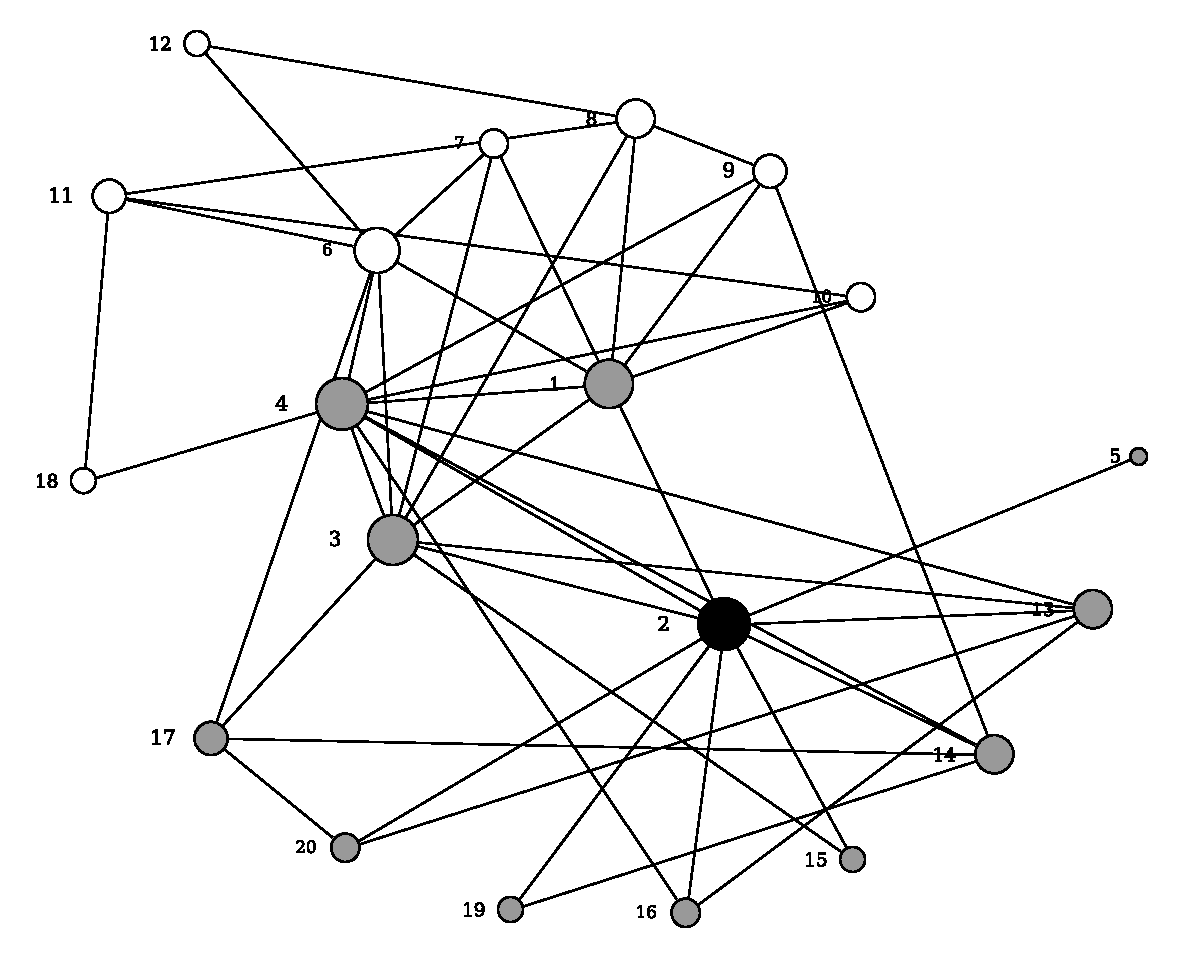
\includegraphics[scale=0.6]{obrazky/colors}%
	}
	\caption{\emph{Príklad prvého kroku pažravého algoritmu.} 
	Vrcholy v grafe majú veľkosť úmernú stupňu (čím väčší stupeň, tým väčší 
	priemer vrchola). V prvom kroku si algoritmus mohol vybrať vrchol 2, čím ho 
	označil ako čierny a jeho susedov (tým dominuje) označil šedou farbou. 
	Bielou sú označené vrcholy, ktoré ešte nie sú dominované čiernymi.}
	\label{img:imp:colors}
\end{figure}


Podľa algoritmu, ktorý je uvedený v časti \ref{sec:greedy} sme implementovali 
algoritmus, ktorý sme označili \alg{greedy}. Podobne sme implementovali aj 
verziu \alg{ch7alg33}. Avšak tá nevyberá vrcholy, ktoré pokrývajú čo najviac 
iných spomedzi šedých a bielych, ale iba z bielych vrcholov. Veľmi podobne je 
implementovaná aj verzia \alg{greedyq}. Jediný rozdiel je, že vrcholy na 
začiatku behu usporiada podľa stupňa od najväčšieho po najmenší.

\subsubsection{Heuristiky na rozhodovanie}

Po troch podobných verziách sme implementovali rôzne heuristiky. Prvou bolo 
odstraňovanie výhonkov. Toto odstraňovanie prebieha na začiatku 
algoritmu, postupne v iteráciách, až kým nie je čo odstrániť. Motiváciou za 
týmto algoritmom je efektívne odstraňovanie ciest. Verzia algoritmu s touto 
heuristikou je označovaná ako \alg{greedysr}. 

V ďalšej verzii sme použili opäť základný pažravý algoritmus, ale ako 
rozhodovací faktor pre výber vrchola sme vybrali počet vrcholov, ktoré po 
vybratí už nebudú mať bieleho suseda (toto nie je to isté ako rád kveta) 
a až potom počet vrcholov, ktorým vrchol dominuje. Motiváciou bolo 
presvedčenie, že často je lepšie vybrať vrchol, ktorý po svojom vybratí čo 
najviac zmenší počet potenciálne vybratých vrcholov v ďalších iteráciách, 
namiesto vyberania vrcholov s najväčším pokrytím.
Heuristika by mala byť nejakým 
kompromisom medzi vyberaním vrcholov "zospodu" a "zvrchu". Táto verzia 
algoritmu je označená ako \alg{greedysw}.

\subsubsection{Zložitejšia heuristika}

Treťou verziou je \alg{floweru}, ktorá je podobná ako \alg{greedysr}, s tým 
rozdielom, že na začiatku spraví iba jeden beh odstraňovania výhonkov. Toto je 
základom pre posledný, zložitejší algoritmus, ktorý je označený \alg{flower}. 

Verzia \alg{flower} na začiatku behu zoradí vrcholy podľa stupňa. Následne sa 
snaží označiť výhonky a kvety. Vyčistí výhonky a upraví graf tak, aby sa mohli 
vybrať kvety. Kvety sa vyberajú postupne. Najviac záleží na ráde kvetu. Ak majú 
nejaké kvety rovnaký rád, tak sa rozhoduje podľa toho, koľko vrcholov po 
vybratí už nebude mať bieleho suseda (podobne ako pri verzii \alg{greedysw}). 
Ak je aj táto hodnota rovnaká, tak zaváži počet bielych susedov (najväčšie 
pokrytie). Ak nepomôže ani toto pravidlo, tak sa vyberie náhodný vrchol.

Po označení výhonkov a kvetov sa začnú označovať zvyšné vrcholy podľa 
jednoduchého pažravého algoritmu. Avšak ako rozhodujúci faktor pri vyberaní 
slúži najprv počet bielych susedov (pokrytie) a potom počet vrcholov, ktoré 
po vybratí už nebudú mať bieleho suseda.

\subsection{Dátové štruktúry a externé knižnice}

Aj keď na porovnanie rôznych algoritmov sú základné dátové štruktúry 
poskytované ako súčasť knižníc jazyka \Java, rozhodli sme sa použiť na 
implementáciu základných dátových štruktúr knižnicu HPPC od poskytovateľa 
Carrot Search Labs vo verzii 0.6.0. Je dostupná na webovej adrese 
\url{http://labs.carrotsearch.com/hppc.html} a licencovaná Apache License 2.0. 
hlavnou výhodou knižnice oproti štandardnej knižnici je menšia spotreba pamäte 
a priamejší prístup k vnútornej reprezentácií (aspoň v danej verzii). To 
spôsobilo celkové zrýchlenie algoritmov a posunulo hranice testovateľných 
grafov.

Aj keď medzi analyzovanými existujúcimi riešeniami je veľa grafových knižníc, 
pripadalo nám jednoduchšie a efektívnejšie implementovať vlastnú reprezentáciu 
grafov pomocou základných prvkov jazyka \Java\ a knižnice HPPC.



\chapter{Dosiahnuté výsledky}\label{chap:vysledky}

V predošlých kapitolách sme spravili prehľad existujúcich algoritmov, popísali 
sme ich implementáciu. V tejto kapitole uvádzame porovnanie jednotlivých 
implementácií. Najprv uvedieme jednotlivé obmedzenia implementácie, potom 
popíšeme spôsob testovania a napokon označenie pre jednotlivé testovacie dáta.

\section{Obmedzenia implementácie}

Vývoj softvéru sa začal na staršom počítači, ktorý má procesor Intel Core 2 
Duo P7350 (2,0GHz dvojjadrový) a 4GB RAM pamäte. Pamäť nebola obmedzením. 
Bohužiaľ počítač 
nebol vhodný na viacvláknové algoritmy, čo spôsobovalo problémy pre algoritmy 
\alg{ch7alg34} a \alg{ch7alg35}. Preto sme sa zamerali na ich jednovláknové 
verzie (\alg{ch7alg34OT}, respektíve \alg{ch7alg35OT}). Heuristiky na pažravý 
algoritmus sa doimplementovali neskôr, preto sa neuvádzajú v starších testoch.

Počas vývoja začal byť dostupný novší počítač, na ktorom sa testovali už všetky 
heuristiky pre pažravý algoritmus. Počítač má procesor Intel Core i5-4690K CPU 
(3,50GHz štvorjadrový) a 16GB pamäte. Tento počítač zvláda viacvláknové 
aplikácie lepšie (o 6 rokov modernejšia architektúra), no 
vzhľadom na zachovanie kompaktnosti sme opäť viacvláknové verzie algoritmov z 
testov vynechali.

Neskoršia práca s externými knižnicami HPPC časy zrýchlila, čo bohužiaľ nie je 
zachované v žiadnej z uvedených tabuliek.

\section{\Java\ verzus \cpp}

Zo začiatku implementácie nebolo jasné, ktorý programovací jazyk bude použitý. 
Ako prvý sa zvolil jazyk \Java. Keďže prevláda povedomie, že interpretovaný 
programovací jazyk (\Java) nemôže byť rýchlejší ako kopmilovaný programovací 
jazyk (\cpp), tak sme sa v priebehu implementácie rozhodli, že skúsime 
naprogramovať niektoré algoritmy aj v jazyku \cpp. Ako vidno z porovnania časov 
behov jednotlivých algoritmov v tabuľkách \ref{table:cpp} a 
\ref{table:java-stare}, jazyk \cpp\ neposkytuje žiadne 
výrazné zrýchlenie. Spolu s faktom, že na porovnanie jednotlivých algoritmov až 
tak rýchlosť netreba, sme sa rozhodli, že budeme pokračovať vo vývoji v jazyku 
\Java.

\section{Spôsob testovania}

Keďže programovací jazyk \Java\ robí optimalizácie kódu počas behu a triedy 
inicializuje "lenivo", tak je potrebné algoritmus spustiť viackrát, aby ukázal 
relevantné výsledky. Algoritmus teda necháme spustiť trikrát a zoberieme tretí 
výsledok. Rozhodnutie je vecou pozorovania. Je kompromisom medzi relevantnými 
výsledkami a dĺžkou skúšania rôznych behov. Z časov nad 20 sekúnd je v 
tabuľkách uvedený iba čas prvého behu algoritmu. 

Rôzne algoritmy sme testovali na rôznych dátach. Najmä podľa toho, aké veľké 
dáta vedeli spracovať v rozumnom čase. Testovacie dáta uvádzame v ďalšej časti.

\section{Testovacie dáta}\label{sec:data}

Testovacie dáta boli grafy rôznych veľkostí a štruktúr. Naše testovacie dáta sa 
dajú rozdeliť do štyroch hlavných skupín. Podľa skupiny majú aj predponu. Sú to 
tieto:

\begin{itemize}
	\item grafy tvorené prioritným pripájaním tvoriace Barabási-Albertov model 
		-- majú predponu \texttt{ba-};
	\item grafy tvorené hranami s náhodnou pravdepodobnosťou vzniku tvoriace 
	náhodný model -- majú predponu \texttt{rnd-};
	\item grafy vytvorené špeciálne podľa obrázka \ref{img:zle1} -- majú 
		predponu \texttt{zle-};
	\item grafy vytvorené z reálnych dát -- majú predponu \texttt{ca-}.
\end{itemize}

Grafové modely sú taktiež popísané aj v časti \ref{sec:modely}. Grafy tvorené 
prioritným pripájaním (podľa Barabási-Albertového modelu) boli 
vytvorené pomocou programu Network Workbench. Ku grafu sa pridali v každom 
kroku tri hrany.
Grafy tvorené náhodnou pravdepodobnosťou vzniku hrán boli taktiež vytvorené 
pomocou programu Network Workbench tak, že hrany sa tvorili s určitou 
pravdepodobnosťou. Táto pravdepodobnosť bola nastavená tak, aby mali grafy 
tvorené náhodne veľmi podobný priemerný stupeň (okolo 6) a teda aj hustotu ako 
grafy vytvorené podľa Barabási-Albertového modelu rovnakej veľkosti. 

Reálne dáta boli prevzaté zo stránky \url{http://snap.stanford.edu/data/} 
\citep{snapnets}. Dáta predstavujú citácie prác ohľadne nejakého vedného oboru. 
Všetky dáta sú spracované zo stránky \url{http://arxiv.org/}. Jednotlivé dáta 
predstavujú spoluprácu v daných oboroch:
\begin{enumerate}
	\item dáta \texttt{ca1} zachytávajú citácie v oblasti všeobecnej teórie relativity;
	\item dáta \texttt{ca2} -- jadrová a subjadrová fyzika;
	\item dáta \texttt{ca22} -- jadrová a subjadrová fyzika, rozšírené;
	\item dáta \texttt{ca3} -- fyzika tuhých látok.
\end{enumerate}

Podľa počtu vrcholov majú názvy jednotlivých grafov príponu. Pre grafy 
vytvorené prioritným pripájaním a náhodné grafy, číslo za predponou vyjadruje 
počet vrcholov grafu. Pre grafy vytvorené podľa obrázka \ref{img:zle1} číslo 
vyjadruje počet vrcholov na "hlavnej" ceste. Pre grafy reálnych dát boli čísla 
zvolené umelo a nemajú žiaden význam. Všetky použité reálne dáta boli siete 
citácií vedeckých publikácií.

\section{Porovnanie algoritmov}

V tejto časti porovnáme medzi sebou jednotlivé skupiny algoritmov. Začneme 
algoritmami dávajúcimi presné výsledky, budeme pokračovať všeobecným porovnaním 
a na koniec zhodnotíme jednotlivé heuristiky pažravého algoritmu.

\subsection{Presné algoritmy}

Do tejto kategórie spadajú algoritmy \alg{naive}, \alg{fnaive} a \alg{fproper}. 
Boli implementované najmä kvôli prehľadu a získaniu veľkostí minimálnych 
dominujúcich množín. Ako vidno zo všetkých tabuliek (\ref{table:java-stare}, 
\ref{table:cpp} a aj \ref{table:java}), pri exaktných algoritmoch nemôžeme 
rátať s tým, že sa dočkáme výsledkov na reálnych dátach.

Môžeme však vidieť, že použitím vhodných úprav vieme posunúť veľkosť grafu, 
kedy vieme vypočítať minimálnu dominujúcu množinu v rozumnom čase, zo zhruba 
20 vrcholov na zhruba 100 vrcholov. Taktiež je dobré všimnúť si, že aj keď 
algoritmus \alg{fproper} používa oveľa zložitejšie výpočty, tak čas behu 
algoritmu to oveľa nezrýchli. Prevedenie na hľadanie maximálneho párenia 
(respektíve minimálneho hranového pokrytia) je teda viac zlepšením teoretickej 
zložitosti ako pomoc reálnemu behu algoritmu.

Celkom zaujímavým je pozorovanie, že na neštruktúrovaných dátach (\texttt{rnd-} 
grafy) mali algoritmy \alg{fnaive} a \alg{fproper} oveľa horší čas ako na 
dátach so štruktúrou (\texttt{ba-} a \texttt{zle-} grafy).

\subsection{Všeobecné porovnanie}

Skôr ako sa pozrieme na celkové hodnotenie, tak sa môžeme pozrieť na algoritmy 
\alg{ch7alg34OT} a \alg{ch7alg35OT}. V tabuľke \ref{table:java-stare} je vidno, 
žo algoritmus \alg{ch7alg35OT} naozaj rieši uvedené problémy v časti 
\ref{sec:dist}. Škoda, že sa nepodarilo vytvoriť prostredie pre distribuovaný 
algoritmus.

Celkovo si môžeme všimnúť (tabuľka \ref{table:java}), že algoritmy bežia 
rýchlejšie na štruktúrovaných dátach (\texttt{ba-} a \alg{zle-}) okrem 
algoritmu \alg{ch7alg33OT}, ktorý beží lepšie na neštruktúrovaných dátach 
(\texttt{rnd-}). 

Keďže štruktúrované aj neštruktúrované dáta majú pomerne rovnakú hustotu hrán, 
tak sme neporovnávali algoritmy na rôzne hustých grafoch.

\subsection{Porovnanie hauristík pažravých algoritmov}

Zatiaľ sme sa pozerali čisto iba na časy. No pri porovnávaní reálnych časov 
pažravých algoritmov nám o rýchlosti veľa prezradí aj veľkosť výslednej 
množiny. Veľkosti výslednej množiny sú uvedené v tabuľke \ref{table:size}. 
Za príklad si môžeme zobrať trebárs základný algoritmus \alg{greedy}. Tam, 
kde mal menšiu výslednú množinu, tam mal aj nižší čas. Napríklad, pre grafy 
\texttt{ba20k} a \texttt{rnd20k} bol rozdiel vo veľkosti nájdených množín 1347. 
To znamená, že sa základný cyklus musel zopakovať oveľa viac krát, čo vyústilo 
do horšieho času algoritmu. Keďže všetky verzie pažravého algoritmu až na 
verziu \alg{flower} mali na začiatku behu algoritmu (pred opakujúcim sa cyklom) 
takmer nulové predpočítavanie rôznych hodnôt, respektíve vyberanie vrcholov do 
výsledku, Tak je tento trend badať na všetkých algoritmoch. 

Algoritmus \alg{flower} je v tomto smere výnimkou. Keďže si predpočítava 
susednosť do vzdialenosti tri a grafy tvorené Barabási-Albertovým modelom sú 
viac spojité ako náhodné grafy, tak sa počet opakovaní následného cyklu prejaví 
až pri grafoch s veľkým počtom vrcholov (v našom prípade \texttt{-20k}).

Keďže v Barabási-Albertovom modely sa každý nový vrchol spojí s práve (v našom 
prípade) dvoma inými, tak nevznikajú výhonky. Taktiež nie je šanca ani na 
vytvorenie kvetov. Takže veľa heuristík založených na odstraňovaní výhonkov a 
kvetov nič neodstráni a teda výsledkom je taká istá množina ako pri základnom 
pažravom algoritme.

\subsection{Porovnanie pažravých algoritmov na reálnych dátach}

V reálnych dátach je situácia iná ako v modelových. V reálnych dátach sa tvoria 
malé lokálne klastre, ktoré sú občas hustejšie prepojené a vytvoria kvet. 
Taktiež je šanca, že nejaký vrchol bude izolovaný alebo takmer izolovaný. Teda 
má zmysel vytvárať heuristiky na základe vyberania výhonkov a kvetov. Keďže 
reálne siete mali nad 5000 vrcholov, iné ako pažravé algoritmy nebolo možné 
testovať. Výsledky testovania sú uvedené v tabuľke \ref{table:real}. 

Algoritmy \alg{ch7alg33} a \alg{greedyq} boli navrhnuté s tým, že budú bežať 
rýchlejšie, ale aj oveľa nepresnejšie, čo sa potvrdilo. Bohužiaľ miera 
nepresnosti na reálnych dátach je príliš veľká na akékoľvek použitie.

Najjednoduchší pažravý algoritmus (\alg{greedy}) dáva 
prekvapivo veľmi dobré výsledky. Je prekonaný iba algoritmom \alg{greedysw}, 
ktorý je rozšírením jednoduchého pažravého algoritmu iba o vhodný spôsob 
výberu vrchola. Najzložitejší, algoritmus \alg{flower}, síce našiel najmenšiu 
dominújúcu množinu spomedzi testovaných algoritmov na dvoch grafoch 
(\texttt{ca1} a \texttt{ca22}), ale mal horšie časy. 

Grafy \texttt{ca22} a \texttt{ca3} sú hustejšie ako ostatné, čo sa prejavilo aj 
na pomalom behu algoritmu \alg{greedysw}.

\section{Tabuľky}

V tejto časti sa nachádzajú tabuľky zobrazujúce výsledky z testovania 
algoritmov. Ich obsah je podrobnejšie rozobratá v predošlých častiach tejto 
kapitoly.

\begin{table}[h]
	\centering
	\caption{Výsledky behov algoritmov v jazyku \cpp\ na staršom počítači.}
	\begin{tabular}{l|rrrr}
		\hline
		& naive & greedy & ch7alg33 & ch7alg34OT \\ \hline
		ba10    & 0     & 0      & 0        & 0          \\
		ba18    & 1     & 0      & 0        & 0          \\
		ba20    & 4,37  & 0      & 0        & 0          \\
		ba100   &       & 0      & 0        & 0          \\
		ba200   &       & 0      & 0,01     & 0,06       \\
		ba1000  &       & 0      & 0        & 1,28       \\
		ba2000  &       & 0,01   & 0,02     & 5,15       \\
		ba10k   &       & 0,08   & 0,51     & 120,32     \\
		ba20k   &       & 0,29   & 2,68     &            \\
		ba100k  &       & 6,52   & 147,56   &            \\
		rnd100  &       & 0      & 0        & 0,03       \\
		rnd200  &       & 0      & 0        & 0,04       \\
		rnd1000 &       & 0      & 0        & 0,21       \\
		rnd10k  &       & 0,07   & 0,53     & 5,6        \\
		zly10   &       & 0      & 0        & 0          \\
		zly20   &       & 0      & 0        & 0,01       \\
		zly100  &       & 0,02   & 0,22     & 4,72       \\ \hline
	\end{tabular}
	\bigskip\par
	V prvom stĺpci je označenie dát (štatistické vlastnosti dát sú v tabuľke 
	\ref{table:stats}) a ku prislušným dátam sú uvedené časy behov pre daný 
	algoritmus (algoritmy sú popísané v kapitole \ref{chap:algoritmy}) v 
	sekundách. Keď si porovnáme výsledné časy s tabuľkou 
	\ref{table:java-stare} zistíme, že prepísanie zdrojového kódu do jazyka 
	\cpp\ neprinieslo výrazné zlepšenie.
	\label{table:cpp}
\end{table}

\begin{table}[h]
	\centering
	\caption{Testovanie rôznych heuristík na dátach z reálneho sveta.}
	\begin{tabular}{l|rrrrrrrr}
		\hline
		         & ca1 - |S| & ca1 - čas & ca2 - |S| & ca2 - čas & ca22 - |S| & ca22 - čas & ca3 - |S| & ca3 - čas \\ \hline
		greedy   & 1176      & 0,124     & 2009      & 0,578     & 2275       & 0,330      & 3694      & 1,311     \\
		ch7alg33 & 1570      & 0,070     & 3243      & 0,121     & 3230       & 0,099      & 5651      & 0,392     \\
		greedyQ  & 1586      & 0,034     & 3239      & 0,087     & 3243       & 0,080      & 5625      & 0,319     \\
		greedysr & 1803      & 0,072     & 3100      & 0,340     & 3667       & 0,118      & 5553      & 0,708     \\
		greedysw & 1159      & 0,348     & 1989      & 1,613     & 2258       & 1,022      & 3649      & 3,548     \\
		floweru  & 1329      & 0,111     & 2131      & 0,511     & 2501       & 0,313      & 3920      & 1,196     \\
		flower   & 1157      & 0,293     & 2018      & 2,406     & 2256       & 0,591      & 3774      & 2,830     \\ \hline
	\end{tabular}
	\bigskip\par
	V prvom stĺpci sú vymenované algoritmy (popísané v kapitole 
	\ref{chap:algoritmy}) a pre daný algoritmus je uvedená veľkosť výslednej 
	nájdenej dominujúcej množiny (stĺpec |S|) a čas, za ktorý algoritmus 
	množinu našiel. Čas je uvedený v sekundách. Štatistické vlastnosti 
	dát sú v tabuľke \ref{table:stats}.
	\label{table:real}
\end{table}

\begin{table}[h]
	\centering
	\caption{Výsledky behov algoritmov v jazyku \Java\ na staršom počítači.}
	\begin{tabular}{l|rrrrrrrr}
		\hline
		& naive & greedy & greedyQ & ch7alg33 & ch7alg34OT & ch7alg35OT & fnaive   & fproper \\ \hline
		ba10    & 0,085 & 0,001  & 0,002   & 0        & 0,003      & 0,004      & 0,008    & 0,009   \\
		ba18    & 1,284 & 0,001  & 0,002   & 0        & 0,013      & 0,008      & 0,035    & 0,035   \\
		ba20    & 4,440 & 0,001  & 0,002   & 0        & 0,011      & 0,008      & 0,049    & 0,047   \\
		ba100   &       & 0,015  & 0,004   & 0,004    & 0,070      & 0,045      & 0,473    & 0,506   \\
		ba200   &       & 0,026  & 0,006   & 0,009    & 0,135      & 0,073      & 30,515   & 30,412  \\
		ba1000  &       & 0,087  & 0,045   & 0,037    & 0,883      & 0,512      &          &         \\
		ba2000  &       & 0,142  & 0,095   & 0,053    & 2,524      & 0,988      &          &         \\
		ba10k   &       & 1,844  & 0,362   & 0,540    & 45,781     & 6,662      &          &         \\
		ba20k   &       & 8,813  & 1,294   & 3,800    &            & 22,256     &          &         \\
		ba100k  &       & 66,762 & 68,669  & 135,197  &            &            &          &         \\
		rnd10   &       & 0,001  & 0,002   &          &            &            & 0,003    & 0,003   \\
		rnd15   &       & 0,001  & 0,002   &          &            &            & 0,048    & 0,043   \\
		rnd20   &       & 0,001  & 0,002   &          &            &            & 0,107    & 0,112   \\
		rnd100  &       & 0,011  & 0,004   &          &            &            & 1293,811 & 1302,940\\
		rnd200  &       & 0,032  & 0,008   &          &            &            &          &         \\
		rnd1000 &       & 0,072  & 0,043   &          &            &            &          &         \\
		rnd2000 &       & 0,114  & 0,096   &          &            &            &          &         \\
		rnd10k  &       & 2,484  & 0,440   &          &            &            &          &         \\
		rnd20k  &       & 11,281 & 1,671   & 4,947    &            &            &          &         \\
		zly10   &       & 0,005  & 0,003   & 0,003    & 0,040      & 0,018      & 0,119    & 0,117   \\
		zly20   &       & 0,022  & 0,010   & 0,022    & 0,098      & 0,036      & 0,809    & 0,814   \\
		zly100  &       & 0,090  & 0,151   & 0,210    & 6,213      & 2,107      &          &         \\ \hline
	\end{tabular}
	\smallskip \par
	V prvom stĺpci je označenie dát (štatistické vlastnosti dát sú v tabuľke 
	\ref{table:stats}) a ku prislušným dátam sú uvedené časy behov pre daný 
	algoritmus (algoritmy sú popísané v kapitole \ref{chap:algoritmy}) v 
	sekundách.
	\label{table:java-stare}
\end{table}

\begin{landscape}

\begin{table}[h]
	\centering
	\caption{Veľkosti nájdených dominujúcich množín pre daný graf a algoritmus.}
\scalebox{0.9}{
		\begin{tabular}{l|rrrrrrrrrrrr}
		\hline
		& naive & greedy & greedyQ & ch7alg33 & greedysr & greedysw & floweru & flower & ch7alg34OT & ch7alg35OT & fnaive & fproper \\ \hline
		ba10    & 2     & 2      & 2       & 2        & 2        & 2        & 2       & 2      & 6          & 6          & 2      & 2       \\
		ba18    & 4     & 4      & 6       & 6        & 5        & 4        & 4       & 4      & 9          & 11         & 4      & 4       \\
		ba20    & 4     & 4      & 7       & 5        & 6        & 4        & 4       & 5      & 10         & 11         & 4      & 4       \\
		ba100   &       & 17     & 33      & 31       & 17       & 17       & 17      & 18     & 54         & 61         & 15     & 15      \\
		ba200   &       & 32     & 59      & 56       & 31       & 35       & 31      & 31     & 102        & 113        & 29     & 29      \\
		ba1000  &       & 142    & 284     & 290      & 147      & 151      & 147     & 146    & 515        & 558        &        &         \\
		ba2000  &       & 276    & 570     & 577      & 273      & 284      & 273     & 274    & 1005       & 1091       &        &         \\
		ba10k   &       & 1393   & 2901    & 2974     & 1391     & 1465     & 1391    & 1390   & 5094       & 5593       &        &         \\
		ba20k   &       & 2828   & 5749    & 5896     & 2828     & 2942     & 2828    & 2817   &            & 11093      &        &         \\
		ba100k  &       & 13947  & 29378   & 29375    & 13947    & 14656    & 13947   & 13928  &            &            &        &         \\
		rnd10   & 2     & 2      & 2       & 2        & 2        & 2        & 2       & 2      & 7          &            & 2      & 2       \\
		rnd15   & 3     & 4      & 3       & 4        & 3        & 3        & 3       & 3      & 10         &            & 3      & 3       \\
		rnd20   & 4     & 4      & 5       & 5        & 4        & 5        & 4       & 4      & 15         &            & 4      & 4       \\
		rnd100  &       & 21     & 28      & 24       & 22       & 22       & 19      & 19     & 62         &            & 18     & 18      \\
		rnd200  &       & 41     & 52      & 53       & 40       & 39       & 40      & 39     & 126        &            &        &         \\
		rnd1000 &       & 201    & 284     & 281      & 202      & 210      & 200     & 199    & 633        &            &        &         \\
		rnd2000 &       & 411    & 541     & 552      & 414      & 411      & 404     & 399    & 1272       &            &        &         \\
		rnd10k  &       & 2083   & 2775    & 2760     & 2122     & 2098     & 2035    & 2024   & 6325       &            &        &         \\
		rnd20k  &       & 4175   & 5560    & 5542     & 4279     & 4193     & 4091    & 4053   &            &            &        &         \\
		zly10   &       & 10     & 35      & 35       & 10       & 10       & 10      & 10     & 10         & 10         & 10     & 10      \\
		zly20   &       & 20     & 120     & 120      & 20       & 20       & 20      & 20     & 20         & 20         & 20     & 20      \\
		zly100  &       & 100    & 2600    & 2600     & 100      & 100      & 100     & 100    & 100        & 100        &        &         \\ \hline
	\end{tabular}
}
	\smallskip \par
	{\footnotesize 
	V prvom stĺpci je označenie dát (štatistické vlastnosti dát sú v tabuľke 
	\ref{table:stats}) a ku prislušným dátam sú uvedené veľkosti nájdených 
	dominujúcich množín pre daný algoritmus (algoritmy sú popísané v kapitole 
	\ref{chap:algoritmy}). Za povšimnutie stojí, že 
	heuristiky určené na siete malého sveta (\alg{greedysw}, \alg{flower}) 
	nenašli typické črty pri grafoch tvorených Barabási-Albertovým modelom 
	(a teda nepriniesli zmenšenie výslednej množiny), 	avšak heuristiky sa 
	prejavili pri reálnych dátach, kde rôzne zmenšili výslednú množinu 
	(tabuľka \ref{table:real}).}
	\label{table:size}
\end{table}

\end{landscape}

\begin{landscape}
\begin{table}[h]
	\centering
	\caption{Výsledky behov algoritmov v jazyku \Java\ na novšom počítači.}
\scalebox{0.9}{
	\begin{tabular}{l|rrrrrrrrrrr}
		\hline
		& naive & greedy & greedyQ & ch7alg33 & greedysr & greedysw & floweru & flower & ch7alg34OT & fnaive  & fproper \\ \hline
		ba10    & 0,010 & 0      & 0       & 0        & 0        & 0        & 0       & 0,001  & 0,001      & 0,001   & 0,001   \\
		ba18    & 0,331 & 0      & 0       & 0        & 0        & 0        & 0       & 0,001  & 0,001      & 0,001   & 0,001   \\
		ba20    & 1,321 & 0      & 0       & 0        & 0        & 0        & 0       & 0,001  & 0,001      & 0,001   & 0,001   \\
		ba100   &       & 0,003  & 0       & 0,002    & 0,001    & 0,003    & 0,001   & 0,004  & 0,016      & 0,084   & 0,145   \\
		ba200   &       & 0,004  & 0       & 0,003    & 0,001    & 0,006    & 0,001   & 0,007  & 0,043      & 15,595  & 15,577  \\
		ba1000  &       & 0,021  & 0,003   & 0,013    & 0,011    & 0,040    & 0,011   & 0,046  & 0,358      &         &         \\
		ba2000  &       & 0,047  & 0,008   & 0,025    & 0,024    & 0,740    & 0,025   & 0,090  & 1,322      &         &         \\
		ba10k   &       & 0,308  & 0,079   & 0,115    & 0,251    & 0,933    & 0,249   & 0,952  & 21,37      &         &         \\
		ba20k   &       & 0,987  & 0,290   & 0,410    & 0,837    & 3,097    & 0,873   & 3,368  &            &         &         \\
		ba100k  &       & 19,602 & 6,831   & 19,201   & 21,315   & 65,587   & 20,743  & 60,146 &            &         &         \\
		rnd10   & 0,011 & 0      & 0       & 0        & 0        & 0        & 0       & 0      & 0          & 0       & 0       \\
		rnd15   & 0,058 & 0      & 0       & 0        & 0        & 0        & 0       & 0      & 0          & 0       & 0       \\
		rnd20   & 1,445 & 0      & 0       & 0        & 0        & 0        & 0       & 0      & 0          & 0,001   & 0,001   \\
		rnd100  &       & 0,003  & 0       & 0        & 0        & 0        & 0       & 0,001  & 0,002      & 634,429 & 631,217 \\
		rnd200  &       & 0,004  & 0       & 0,001    & 0        & 0,001    & 0       & 0,002  & 0,008      &         &         \\
		rnd1000 &       & 0,019  & 0,001   & 0,007    & 0,004    & 0,015    & 0,004   & 0,016  & 0,105      &         &         \\
		rnd2000 &       & 0,045  & 0,004   & 0,020    & 0,013    & 0,048    & 0,013   & 0,048  & 0,303      &         &         \\
		rnd10k  &       & 0,384  & 0,101   & 0,120    & 0,294    & 0,984    & 0,313   & 0,929  & 2,827      &         &         \\
		rnd20k  &       & 1,337  & 0,390   & 0,478    & 1,224    & 3,833    & 1,260   & 3,703  &            &         &         \\
		zly10   &       & 0      & 0       & 0        & 0        & 0        & 0       & 0      & 0          & 0       & 0       \\
		zly20   &       & 0      & 0       & 0        & 0        & 0        & 0       & 0,001  & 0,001      & 0,009   & 0,006   \\
		zly100  &       & 0,027  & 0,016   & 0,037    & 0,003    & 0,100    & 0,011   & 0,088  & 0,662      &         &         \\ \hline
	\end{tabular}
}
	\smallskip \par
	{\footnotesize
	V prvom stĺpci je označenie dát (štatistické vlastnosti dát sú v tabuľke 
	\ref{table:stats}) a ku prislušným dátam sú uvedené veľkosti nájdených 
	dominujúcich množín pre daný algoritmus (algoritmy sú popísané v kapitole 
	\ref{chap:algoritmy}). Oproti tabuľke \ref{table:java-stare} vidno 
	zrýchlenie vďaka výkonnejšiemu počítaču. V kombinácií s veľkosťou nájdenej 
	výslednej množiny (tabuľka \ref{table:size}) si môžeme všimnúť, ako čas 
	pažravých algoritmov závisí od veľkosti nájdenej množiny (algoritmy 
	\alg{greedy-} a \alg{flower-} a porovnanie \texttt{ba-} oproti \texttt{rnd-} 
	dátam rovnakej veľkosti).}
	\label{table:java}
\end{table}
\end{landscape}

\begin{landscape}
	\centering
\begin{table}[h]
	\centering
	\caption{Štatistické údaje dát.}
\scalebox{0.9}{
		\begin{tabular}{l|rrrrrrr}
		\hline
		& počet vrcholov & počet hrán & priemerný stupeň & hustota & priemerný klasterizačný koeficient & priemer & priemerná najkratšia cesta \\ \hline
		ba10    & 10             & 20         & 4                & 0,444   & 0,673                              & 3       & 1,667                      \\
		ba18    & 18             & 41         & 4,556            & 0,268   & 0,421                              & 4       & 1,948                      \\
		ba20    & 20             & 46         & 4,6              & 0,242   & 0,412                              & 4       & 2,016                      \\
		ba100   & 100            & 279        & 5,58             & 0,056   & 0,167                              & 5       & 2,622                      \\
		ba200   & 200            & 574        & 5,74             & 0,029   & 0,088                              & 5       & 2,909                      \\
		ba1000  & 1000           & 2964       & 5,928            & 0,005   & 0,028                              & 6       & 3,534                      \\
		ba2000  & 2000           & 5962       & 5,962            & 0,003   & 0,019                              & 6       & 3,766                      \\
		ba10k   & 10000          & 29950      & 5,99             & 0,006   & 0,006                              & 7       & 4,306                      \\
		ba20k   & 20000          & 59943      & 5,994            & 0,0003  & 0,003                              & 7       & 4,53                       \\
		ba100k  & 100000         & 299921     & 5,998            & 0,00006 & 0,0008                             & 8       & 5,039                      \\
		rnd10   & 10             & 30         & 6                & 0,667   & 0,742                              & 3       & 1,356                      \\
		rnd15   & 15             & 45         & 6                & 0,429   & 0,417                              & 3       & 1,59                       \\
		rnd20   & 20             & 60         & 6                & 0,316   & 0,262                              & 3       & 1,732                      \\
		rnd100  & 100            & 301        & 6,02             & 0,061   & 0,053                              & 5       & 2,746                      \\
		rnd200  & 200            & 601        & 6,01             & 0,03    & 0,033                              & 6       & 3,142                      \\
		rnd1000 & 1000           & 3000       & 6                & 0,006   & 0,006                              & 8       & 4,059                      \\
		rnd2000 & 2000           & 6042       & 6,042            & 0,003   & 0,003                              & 8       & 4,421                      \\
		rnd10k  & 10000          & 30000      & 6                & 0,006   & 0,0006                             & 11      & 5,351                      \\
		rnd20k  & 20000          & 60036      & 6,004            & 0,0003  & 0,0003                             & 11      & 5,73                       \\
		zly10   & 76             & 75         &                  &         &                                    &         &                            \\
		zly20   & 251            & 250        &                  &         &                                    &         &                            \\
		zly100  & 5251           & 5250       &                  &         &                                    &         &                            \\
		ca1     & 5242           & 28980      & 11,057           &         &                                    & 17      & 6,047                      \\
		ca2     & 12008          & 237010     & 39,475           &         & 0,696                              & 13      & 2,622                      \\
		ca22    & 9877           & 51971      & 10,524           &         &                                    & 18      & 5,945                      \\
		ca3     & 23133          & 186936     & 16,162           &         & 0,65                               & 15      &                            \\ \hline
	\end{tabular}
	}
	\smallskip\par
	{\footnotesize V tejto tabuľke sú uvedené základné štatistické údaje dát, 
		s ktorými sme pracovali. V prvom stĺpci je názov dát. Predpona 
		\texttt{ba-} patrí grafom podľa Barabási-Albertoveho modelu, predponou 
		\texttt{rnd-} sú označené grafy vytvorené náhodným modelom, predponou 
		\texttt{zly-} sú označené grafy vytvorené podľa obrázka \ref{img:zle1} 
		a predponu \texttt{ca-} majú reálne dáta (vo všetkých prípadoch je to 
		sieť vedeckých publikácií). Dáta sú popísané aj v časti \ref{sec:data}.}
	\label{table:stats}
\end{table}
\end{landscape}

\backmatter
\cleardoublepage
\phantomsection
\addcontentsline{toc}{chapter}{Záver}
\chapter*{Záver}\label{chap:zaver}

V práci sme sa snažili naplniť ciele zadania. A to spraviť prehľad algoritmov 
hľdajúcich minimálne dominujúce množiny a skúsiť vylepšiť niektoré algoritmy, 
ktoré hľadajú minimálne dominujúce množiny na sieťach malého sveta. 

V kapitole \ref{chap:definicie} sme popísali základné pojmy a uviedli čitateľa 
do problematiky grafov, komplexných sietí a hľadania minimálnej dominujúcej 
množiny. Kapitolu \ref{chap:algoritmy} sme začali spísaním prehľadu súčasných 
základných existujúcich algoritmov na hľadanie minimálnej dominujúcej množiny. 
Ďalej sme v tejto kapitole načrtli výhody v prípade, že vstupným grafom je 
komplexná sieť. Nakoniec sme navrhli niekoľko heuristík, o ktorých sme 
predpokladali, že nejako zlepšia čas behu alebo výsledky algoritmov. Keďže 
sme sa v práci chceli zaoberať dátami z reálneho sveta, zvolili sme si 
heuristiky na zlepšenie tých algoritmov, ktoré majú šancu spracovať také veľké 
dáta.

V kapitolách \ref{chap:popis} a \ref{chap:implementacia} sme popísali návrh a 
implementáciu softvéru. Preskúmali sme existujúce riešenia a na základe analýzy 
navrhli, ako by mala implementačná časť práce vyzerať.
Softvér nakonie nenadväzoval na žiadne predošlé práce, aj keď 
používal pomocnú knižnicu (HPPC) na uchovanie základných dátových štruktúr. 
V konečnom dôsledku malo použitie externej knižnice pozitívny dopad. 
Implementačnú časť práce sme sa rozhodli spraviť samostatne a nenadväzovať 
kvôli úzkej špecifikácií algoritmov a pohodlnosti práce s vlastnými 
zložitejšími dátovými a programovými štruktúrami oproti existujúcim riešeniam.

V kapitole \ref{chap:vysledky} sme opísali výsledky z implementácie softvéru a 
porovnali sme algoritmy medzi sebou a na rôznych dátach, včetne reálnych sietí 
citácií. Z navrhovaných heuristík mala každá svoje slabé a silné miesta. 
Čo dáva priestor na ďalšie zlepšovania. 

Veľmi potešujúce však je, že sme našli heuristiku, ktorá na všetkých 
testovaných reálnych dátach prekonala veľkosťou dominujúcej množiny 
jednoduchý pažravý algoritmus (verzia \alg{greedysw}). Iba o trochu viac 
sofistikovaný spôsob vyberania (uprednostňuj vrcholy, ktoré svojím vybratím 
čo najviac zmenšia množinu vrcholov, ktoré majú nejakého bieleho suseda) 
dosiahol zlepšenie. Zlepšenie sa nepodarilo vždy pri algoritme so zložitejšou 
štruktúrou -- verzii \alg{flower}.
Tento výsledok odráža skutočnosť, že často algoritmy s 
jednoduchou štruktúrou bývajú tým najvhodnejším riešením.

V tejto práci sme nevyužili vedomosť, že siete malého sveta sú síce odolné voči 
náhodným útokom, no zraniteľné cielenými útokmi v tom zmysle, že ich vieme 
odobratím malého počtu hrán rozdeliť na viacero komponentov. Je možné, že keby 
sme vedeli, tieto hrany efektívne určiť, mohli by sme skúmať, ako dôležité sú 
vrcholy, ktoré sú incidentné s hranou a na základe toho ich prioritne ne/vybrať 
do výslednej množiny.

Vďaka tomu, že vieme, že siete malého sveta sú riedke grafy, môžeme tieto grafy 
rozdeliť na množinu stromov, na ktorých sa minimálna dominujúca množina hľadá 
ľahšie. Je však otázne, ako vyriešiť vrcholy, v ktorých tieto stromy v pôvodnom 
grafe susedia. Aj keď sa tento prístup zdá byť prijateľný, tak vieme, že siete 
malého sveta majú veľa lokálnych klastrov a pridelení týchto klastrov by 
vznikalo veľa stromov, čo by mohlo viesť ku vybratiu veľa "zbytočných" 
vrcholov. Vďaka tejto komplikácií a tomu, že sa tento spôsob riešenia výrazne 
odlišuje od zvyšných, sme takýto postup hľadania minimálnej dominujúcej množiny 
nakoniec vynechali.

V ďalšej činnosti je teda vhodné zamerať sa podrobnejšie na to, aké heuristiky 
dávajú lepšie výsledky pre rôzne typy dát ako napríklad hustejšie/redšie grafy, 
grafy s väčšou/menšou klasterizáciou alebo trebárs rôzne spôsoby vyberania 
výhonkov. To by umožňovalo vzniku možno lepšej heuristiky (či už z pohľadu času 
alebo veľkosti nájdenej množiny) alebo kombinovaného algoritmu s využitím 
viacerých heuristík (podobne ako naša verzia \alg{flower}). Taktiež je vhodné 
zamerať sa na dobré implementovanie distribuovaných algoritmov. Buď vylepšiť 
algoritmy \alg{ch7alg34} a \alg{ch7alg35} tým, že lepšie využijeme nejaké 
distribuované prostredie alebo skúsiť rozobrať distribuovanú verziu vynechaného 
algoritmu rozdelenia grafu na stromy. Taktiež by v ďalšej práci bolo vhodné 
výsledky vizualizovať. Vhodná vizualizácia by mohla pomôcť pri odstraňovaní 
slabých miest heuristík a priniesť veľa podnetov na tvorbu ďalších heuristík.


\cleardoublepage
\phantomsection
\addcontentsline{toc}{chapter}{Literatúra}

\printbibliography

\backmatter

\newpage
\pagestyle{empty}
\hbox{}
 
\end{document}

